% !TEX root = main.tex

\section{Data distributions}

\renewcommand{\thefigure}{M.\arabic{figure}}

\subsection*{Comparison of signal and calibration channels}

\begin{figure}[h]
\centering
\includegraphics[height=!,width=0.3\textwidth]{figs/dataVsMC/norm2signal/Ds2all_Bs_PT.pdf}
\includegraphics[height=!,width=0.3\textwidth]{figs/dataVsMC/norm2signal/Ds2all_Bs_ETA.pdf}
\includegraphics[height=!,width=0.3\textwidth]{figs/dataVsMC/norm2signal/Ds2all_NTracks.pdf}

%\includegraphics[height=!,width=0.4\textwidth]{figs/dataVsMC/norm2signal/Ds2all_Bs_FDCHI2_OWNPV.pdf}
%\includegraphics[height=!,width=0.4\textwidth]{figs/dataVsMC/norm2signal/Ds2all_Bs_DTF_MERR.pdf}

\includegraphics[height=!,width=0.3\textwidth]{figs/dataVsMC/norm2signal/Ds2all_Bs_BsDTF_TAUERR.pdf}
\includegraphics[height=!,width=0.3\textwidth]{figs/dataVsMC/norm2signal/Ds2all_OS_Combination_PROB.pdf}
\includegraphics[height=!,width=0.3\textwidth]{figs/dataVsMC/norm2signal/Ds2all_SS_Kaon_PROB.pdf}

%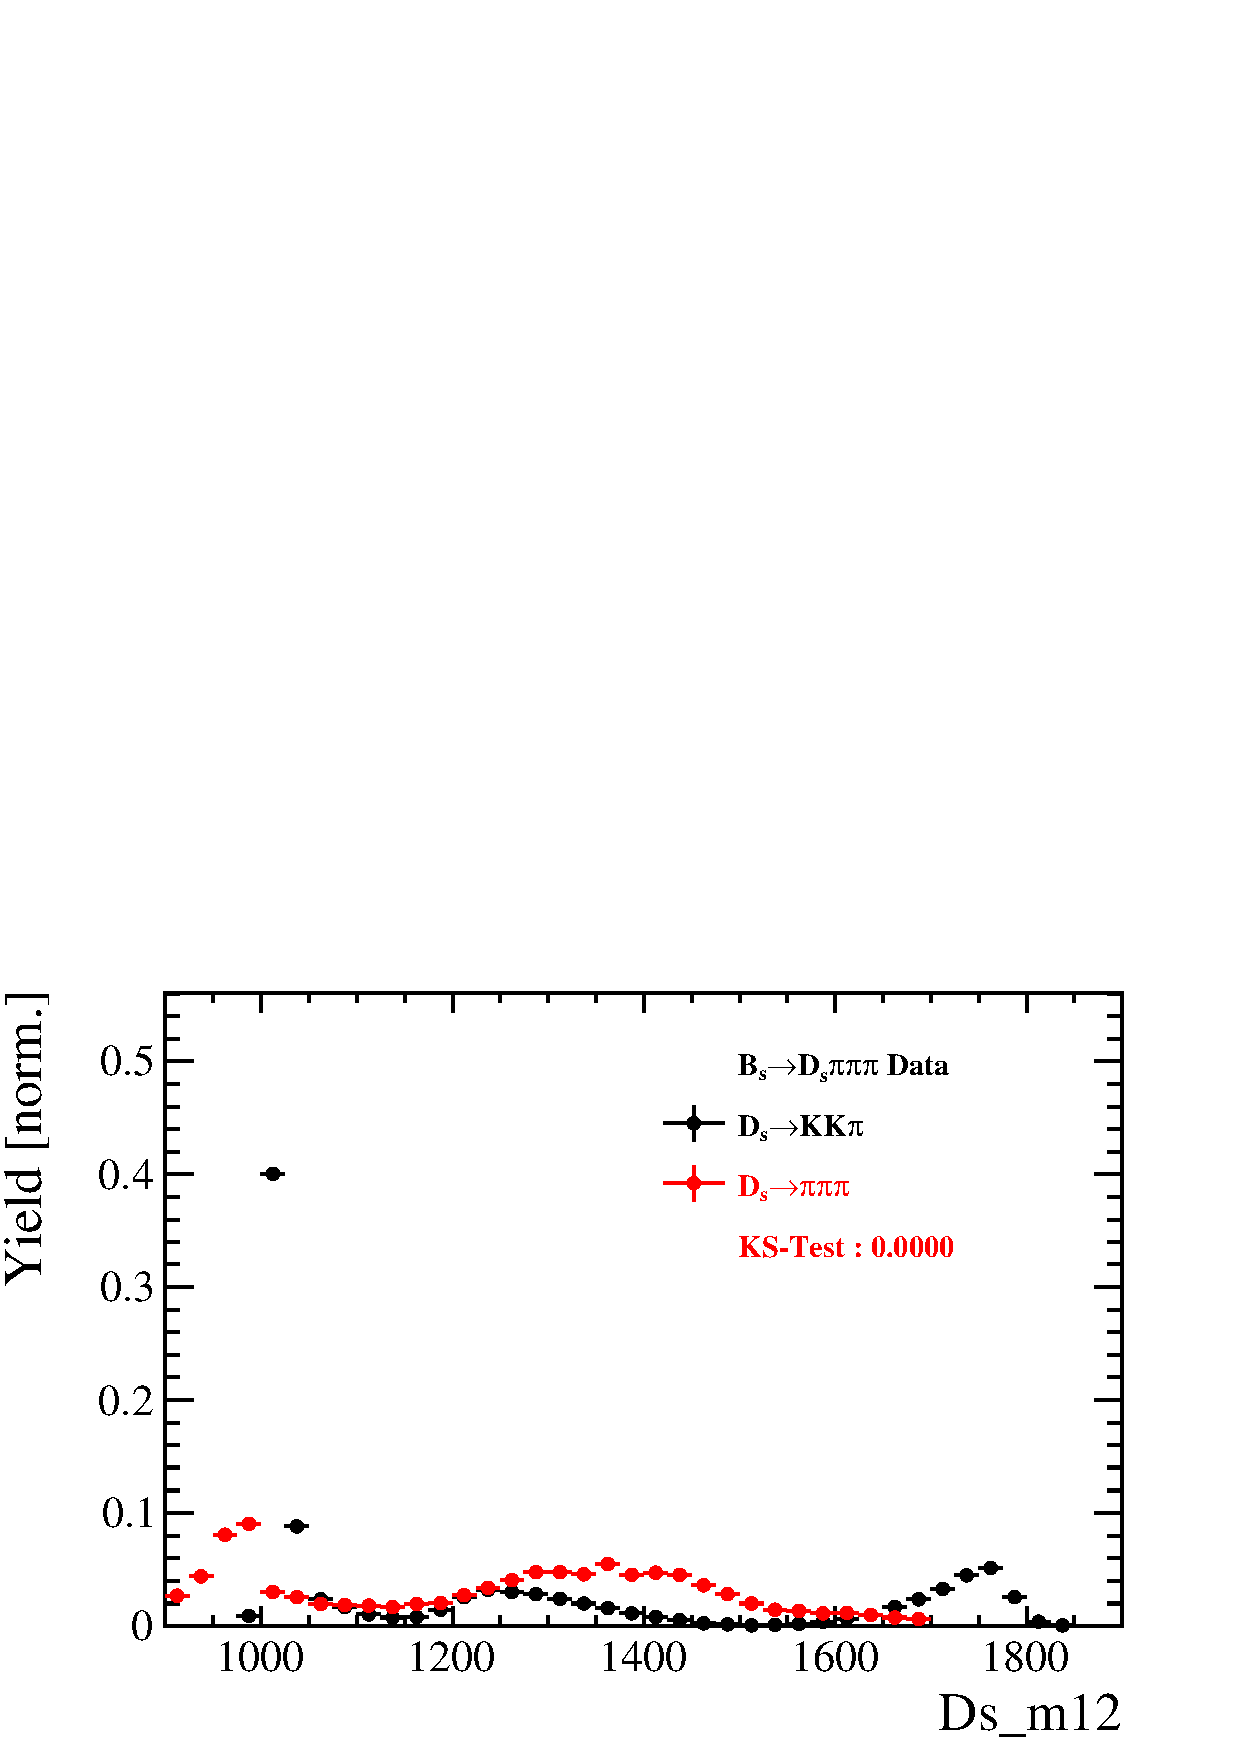
\includegraphics[height=!,width=0.4\textwidth]{figs/dataVsMC/norm2signal/Ds2all_Ds_m12.pdf}
%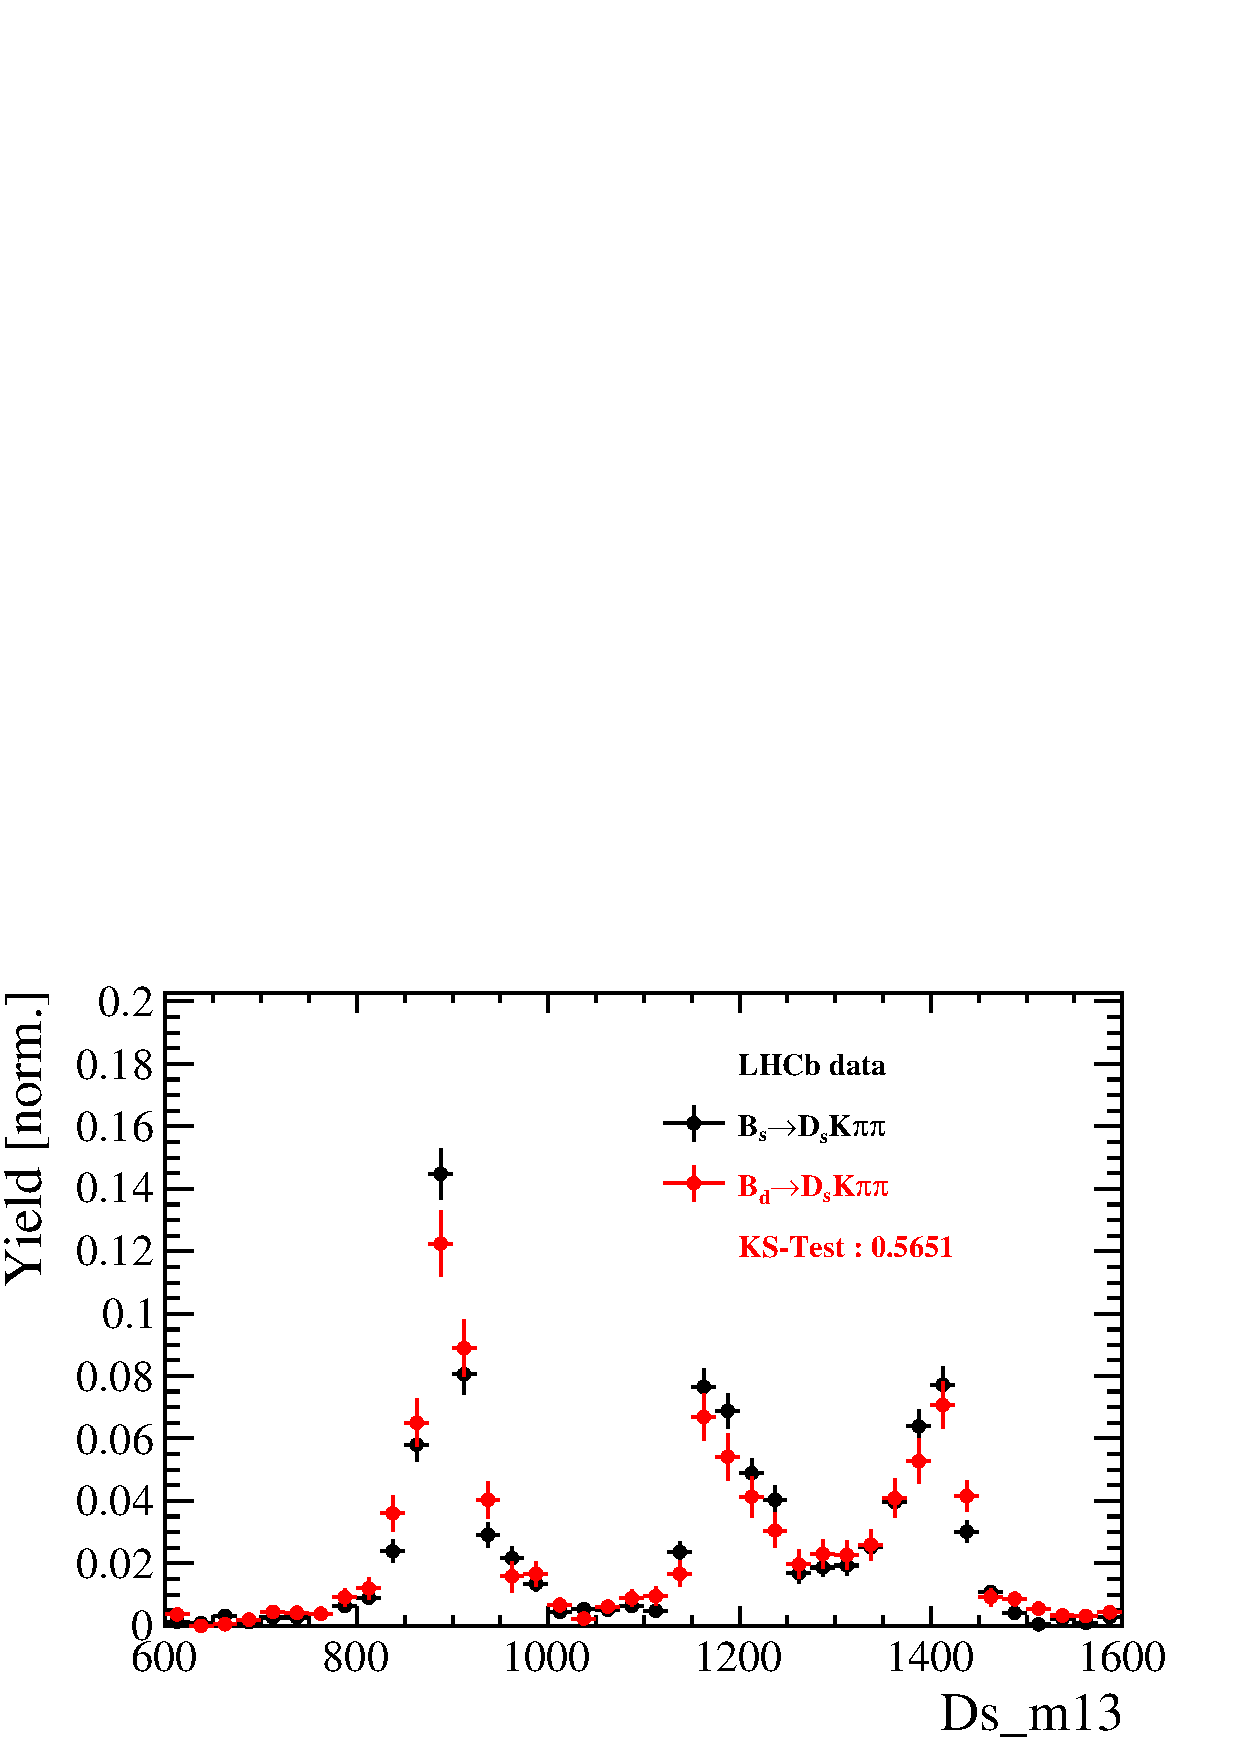
\includegraphics[height=!,width=0.4\textwidth]{figs/dataVsMC/norm2signal/Ds2all_Ds_m13.pdf}

\caption{Comparison between $B_s \to D_s K \pi \pi$ and $B_s \to D_s \pi \pi \pi$ decays for selected variables.}
\label{fig:}

\includegraphics[height=!,width=0.3\textwidth]{figs/dataVsMC/B0vsBs_signal/Ds2all_Bs_PT.pdf}
\includegraphics[height=!,width=0.3\textwidth]{figs/dataVsMC/B0vsBs_signal/Ds2all_Bs_ETA.pdf}
\includegraphics[height=!,width=0.3\textwidth]{figs/dataVsMC/B0vsBs_signal/Ds2all_NTracks.pdf}

\includegraphics[height=!,width=0.3\textwidth]{figs/dataVsMC/B0vsBs_signal/Ds2all_Bs_BsDTF_TAUERR.pdf}
%\includegraphics[height=!,width=0.4\textwidth]{figs/dataVsMC/B0vsBs_signal/Ds2all_Bs_DTF_MERR.pdf}
\includegraphics[height=!,width=0.3\textwidth]{figs/dataVsMC/B0vsBs_signal/Ds2all_OS_Combination_PROB.pdf}
\includegraphics[height=!,width=0.3\textwidth]{figs/dataVsMC/B0vsBs_signal/Ds2all_SS_Kaon_PROB.pdf}

\caption{Comparison between $B_s \to D_s K \pi \pi$ and $B_d \to D_s K \pi \pi$ decays for selected variables.}

\end{figure}

%\begin{figure}[h]
%\centering
%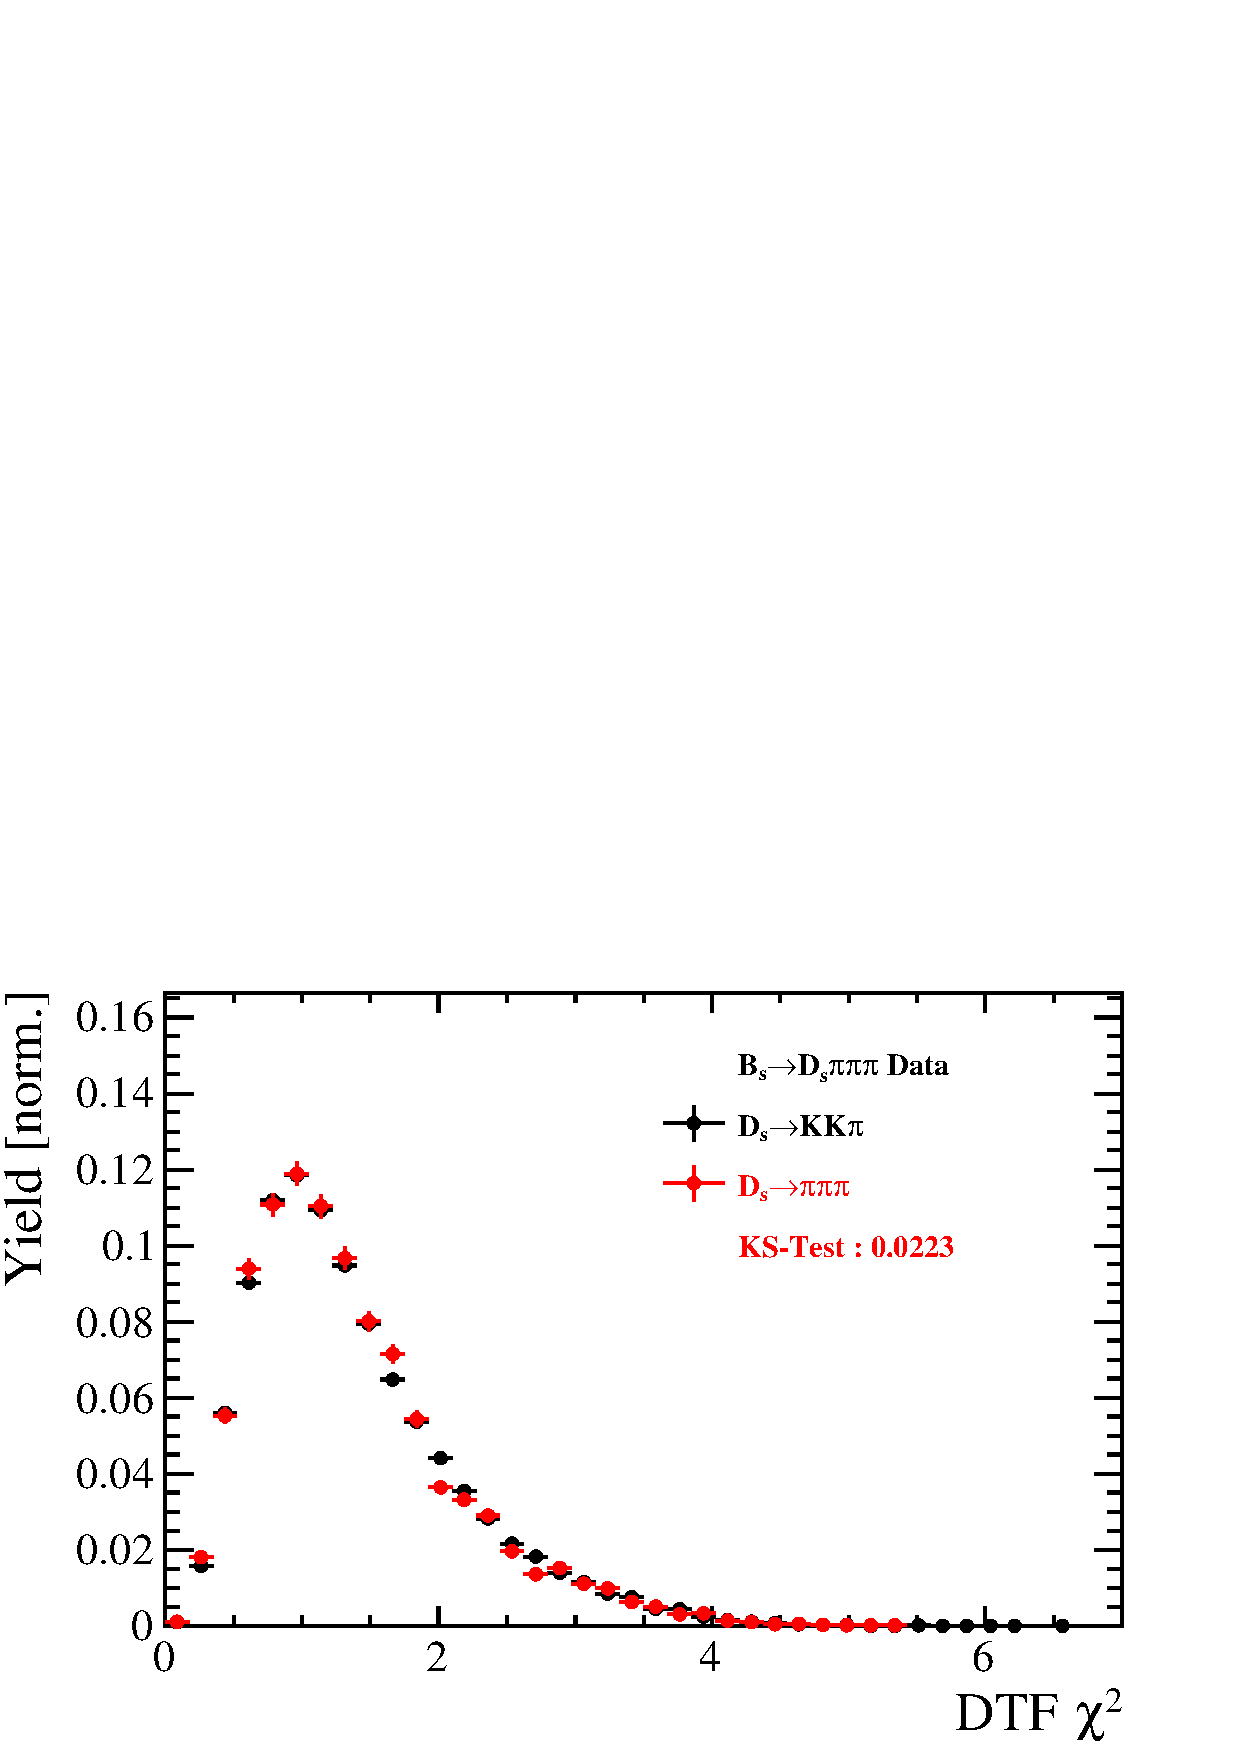
\includegraphics[height=!,width=0.4\textwidth]{figs/dataVsMC/norm2signal/Ds2all_DTF_CHI2NDOF.pdf}
%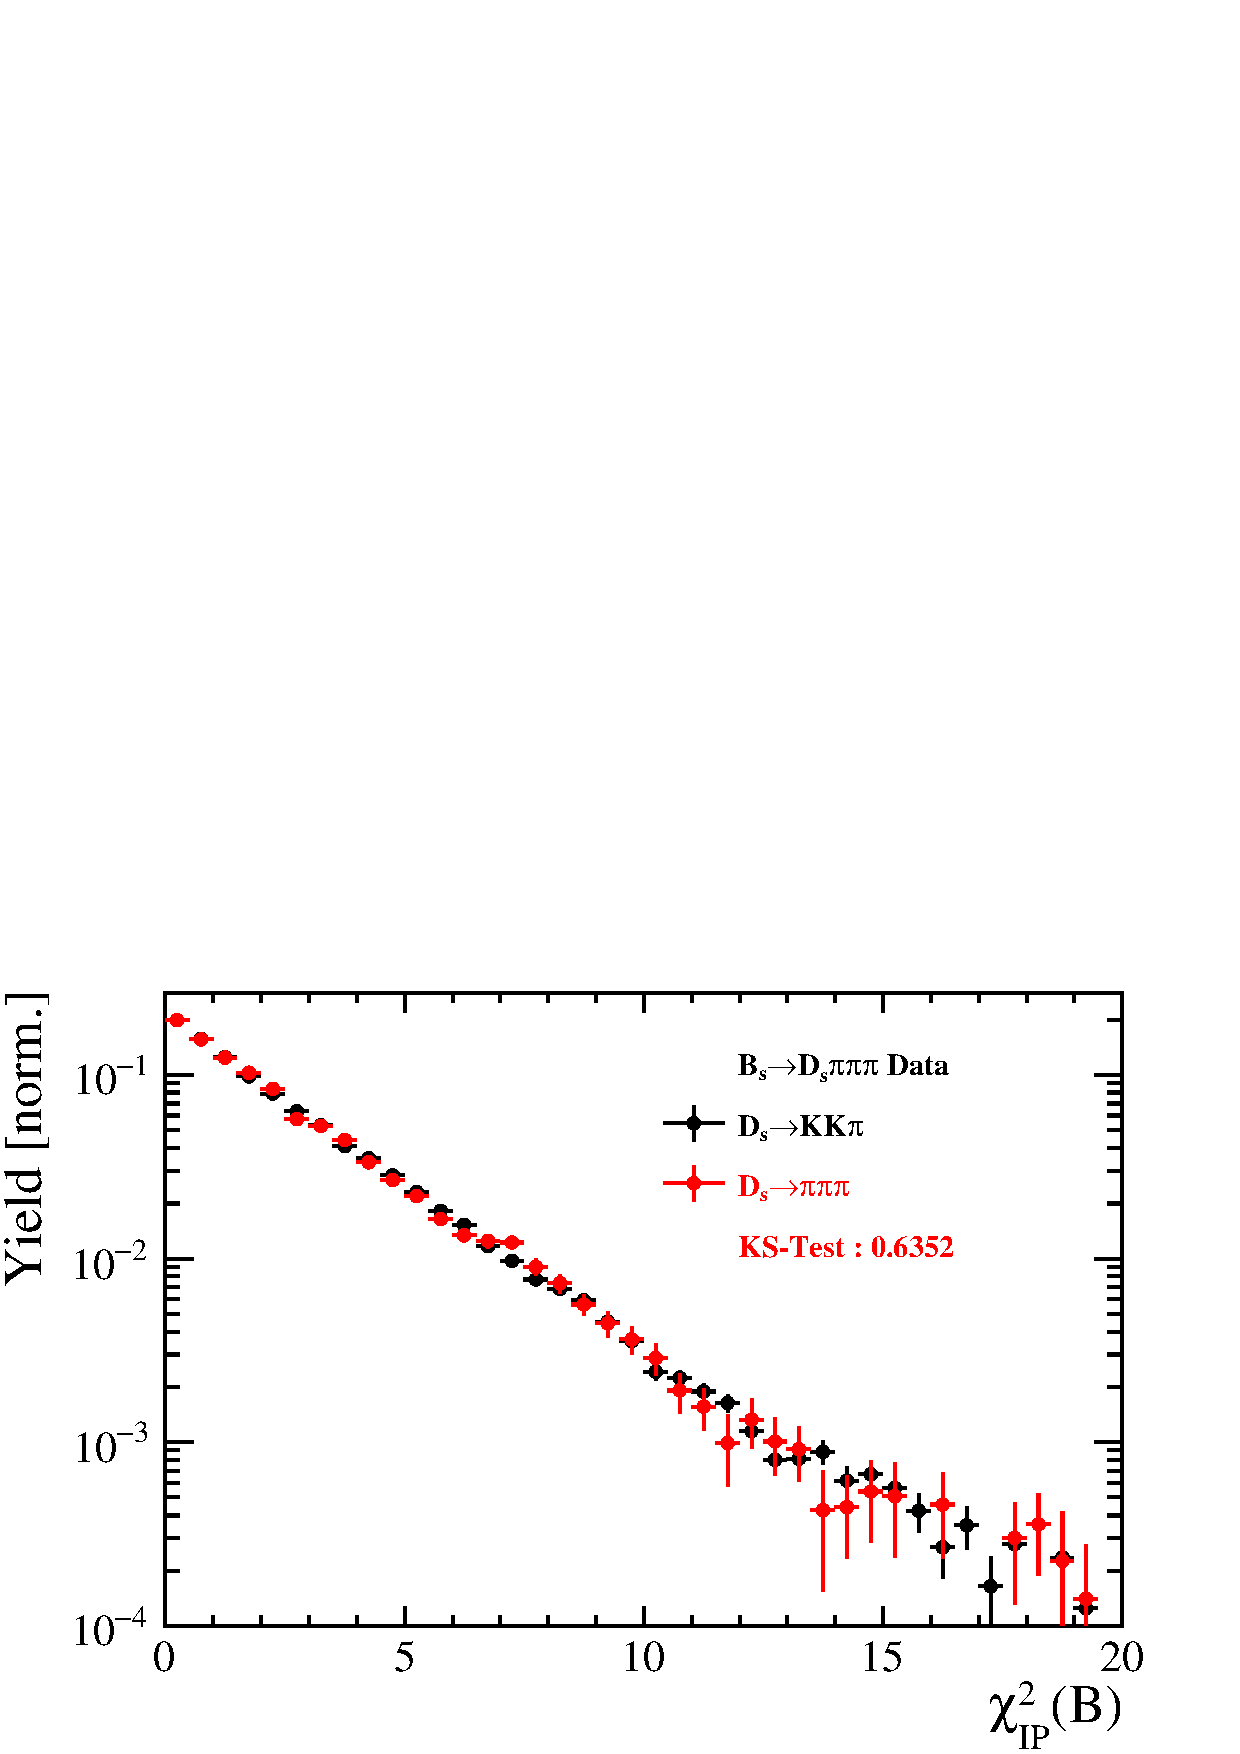
\includegraphics[height=!,width=0.4\textwidth]{figs/dataVsMC/norm2signal/Ds2all_Bs_IPCHI2_OWNPV.pdf}
%
%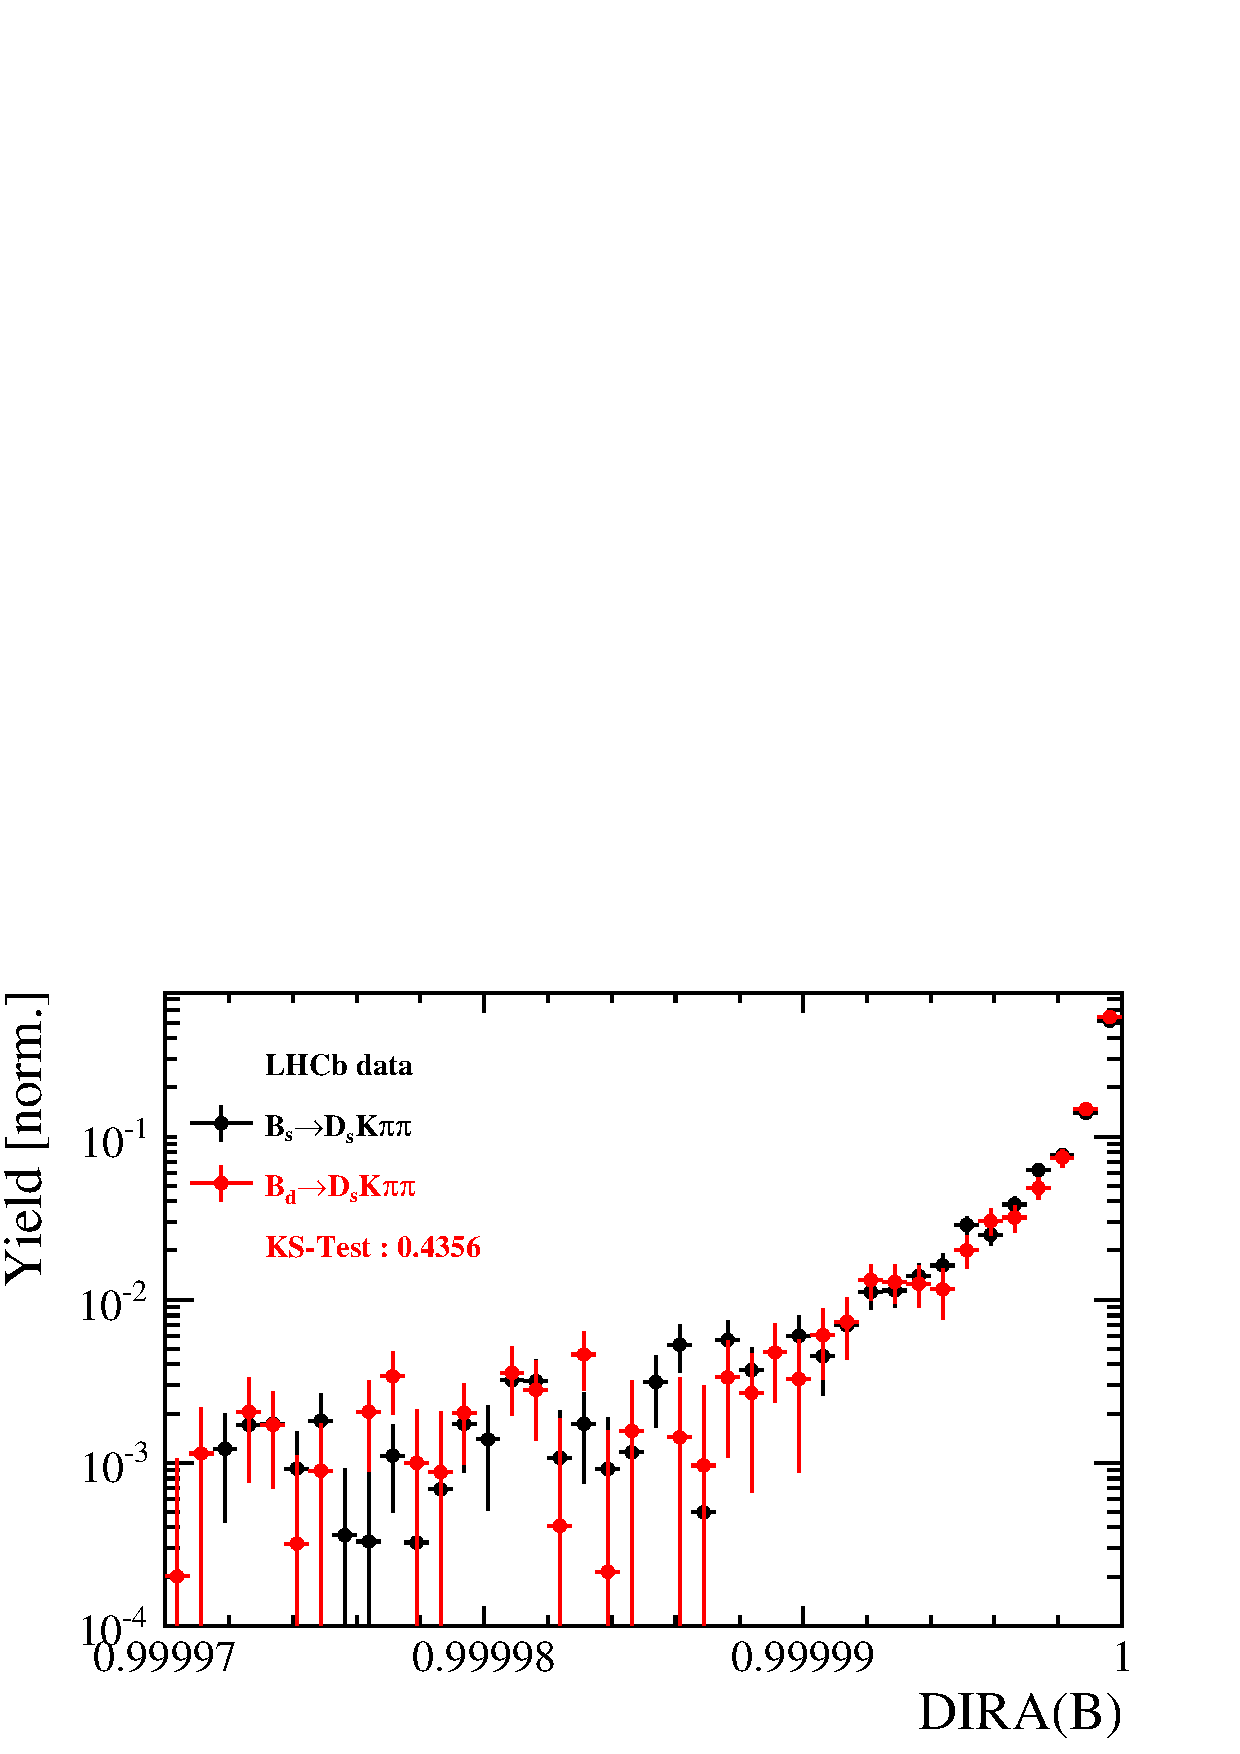
\includegraphics[height=!,width=0.4\textwidth]{figs/dataVsMC/norm2signal/Ds2all_Bs_DIRA_OWNPV.pdf}
%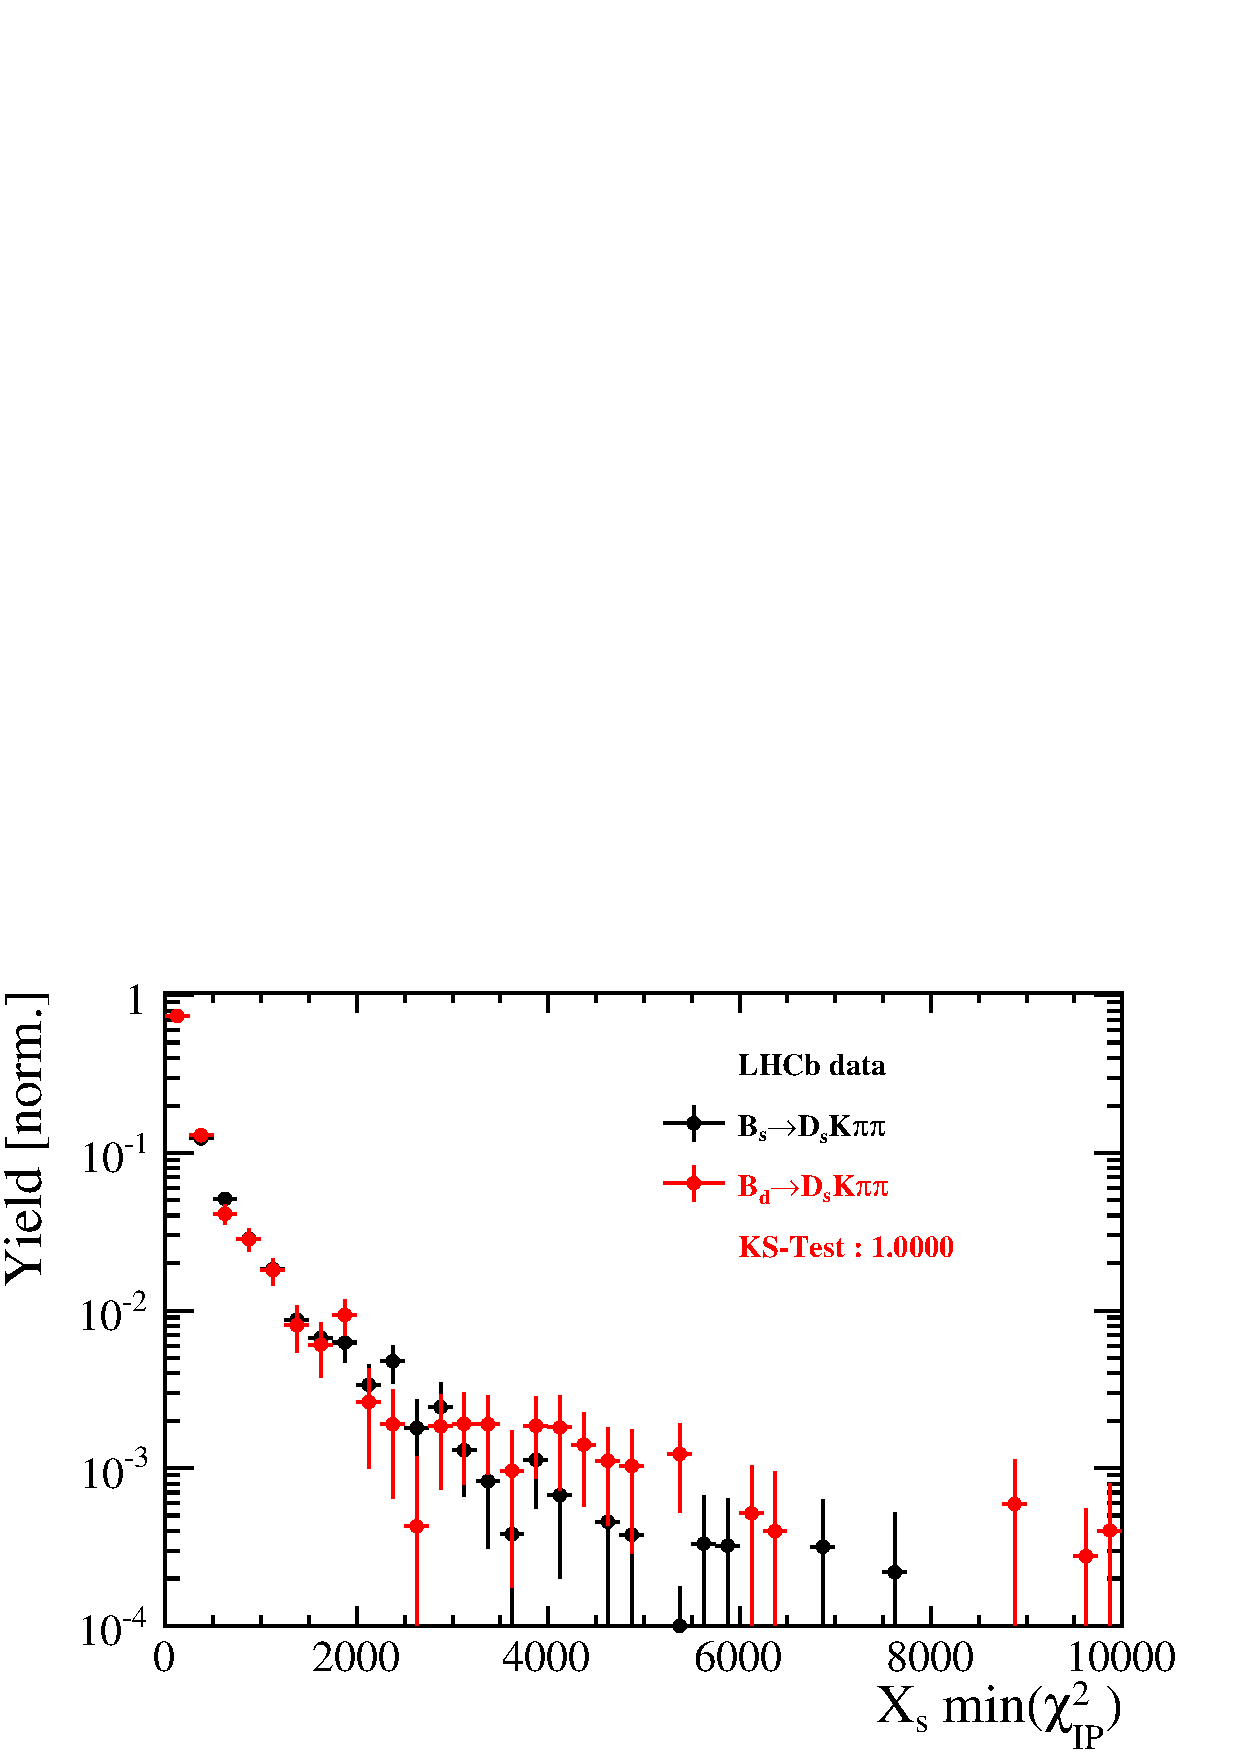
\includegraphics[height=!,width=0.4\textwidth]{figs/dataVsMC/norm2signal/Ds2all_XsDaughters_min_IPCHI2.pdf}
%
%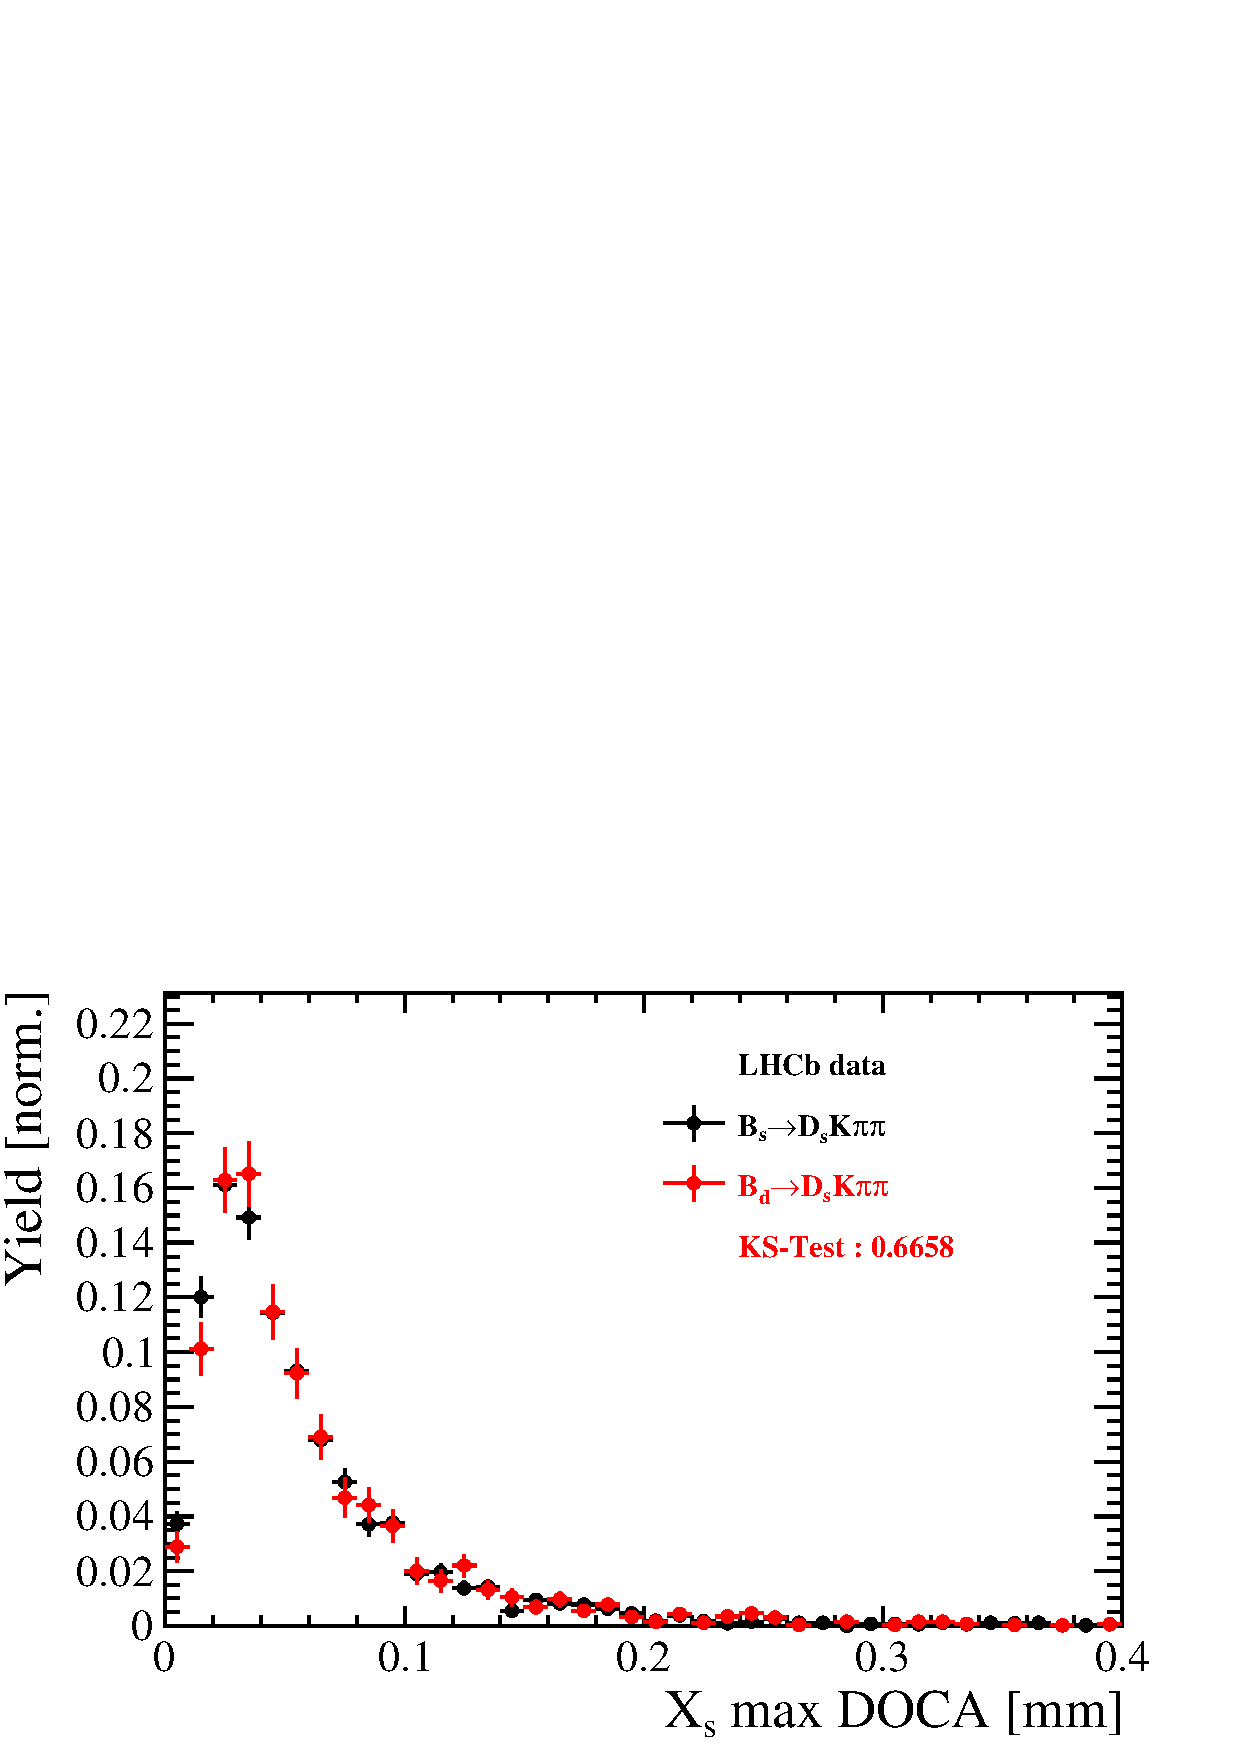
\includegraphics[height=!,width=0.4\textwidth]{figs/dataVsMC/norm2signal/Ds2all_Xs_max_DOCA.pdf}
%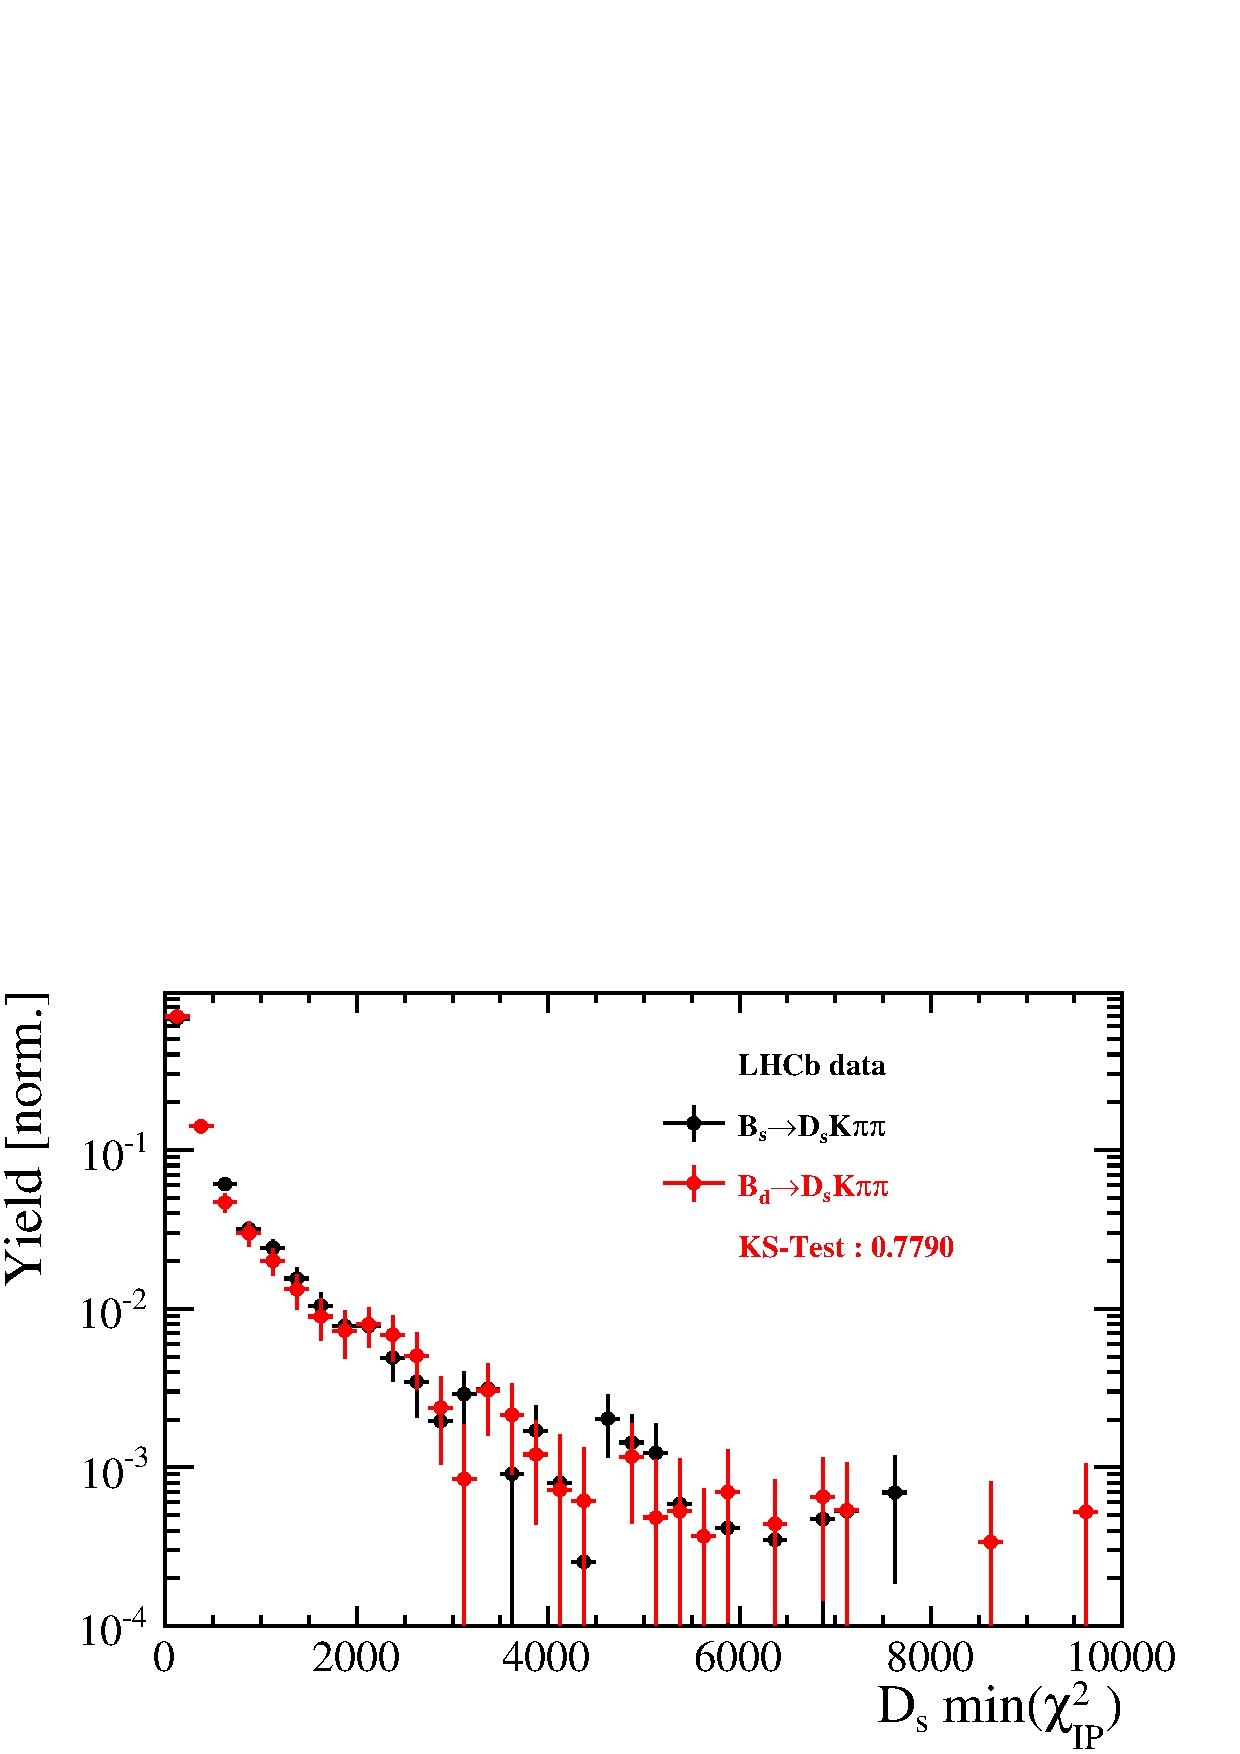
\includegraphics[height=!,width=0.4\textwidth]{figs/dataVsMC/norm2signal/Ds2all_DsDaughters_min_IPCHI2.pdf}
%
%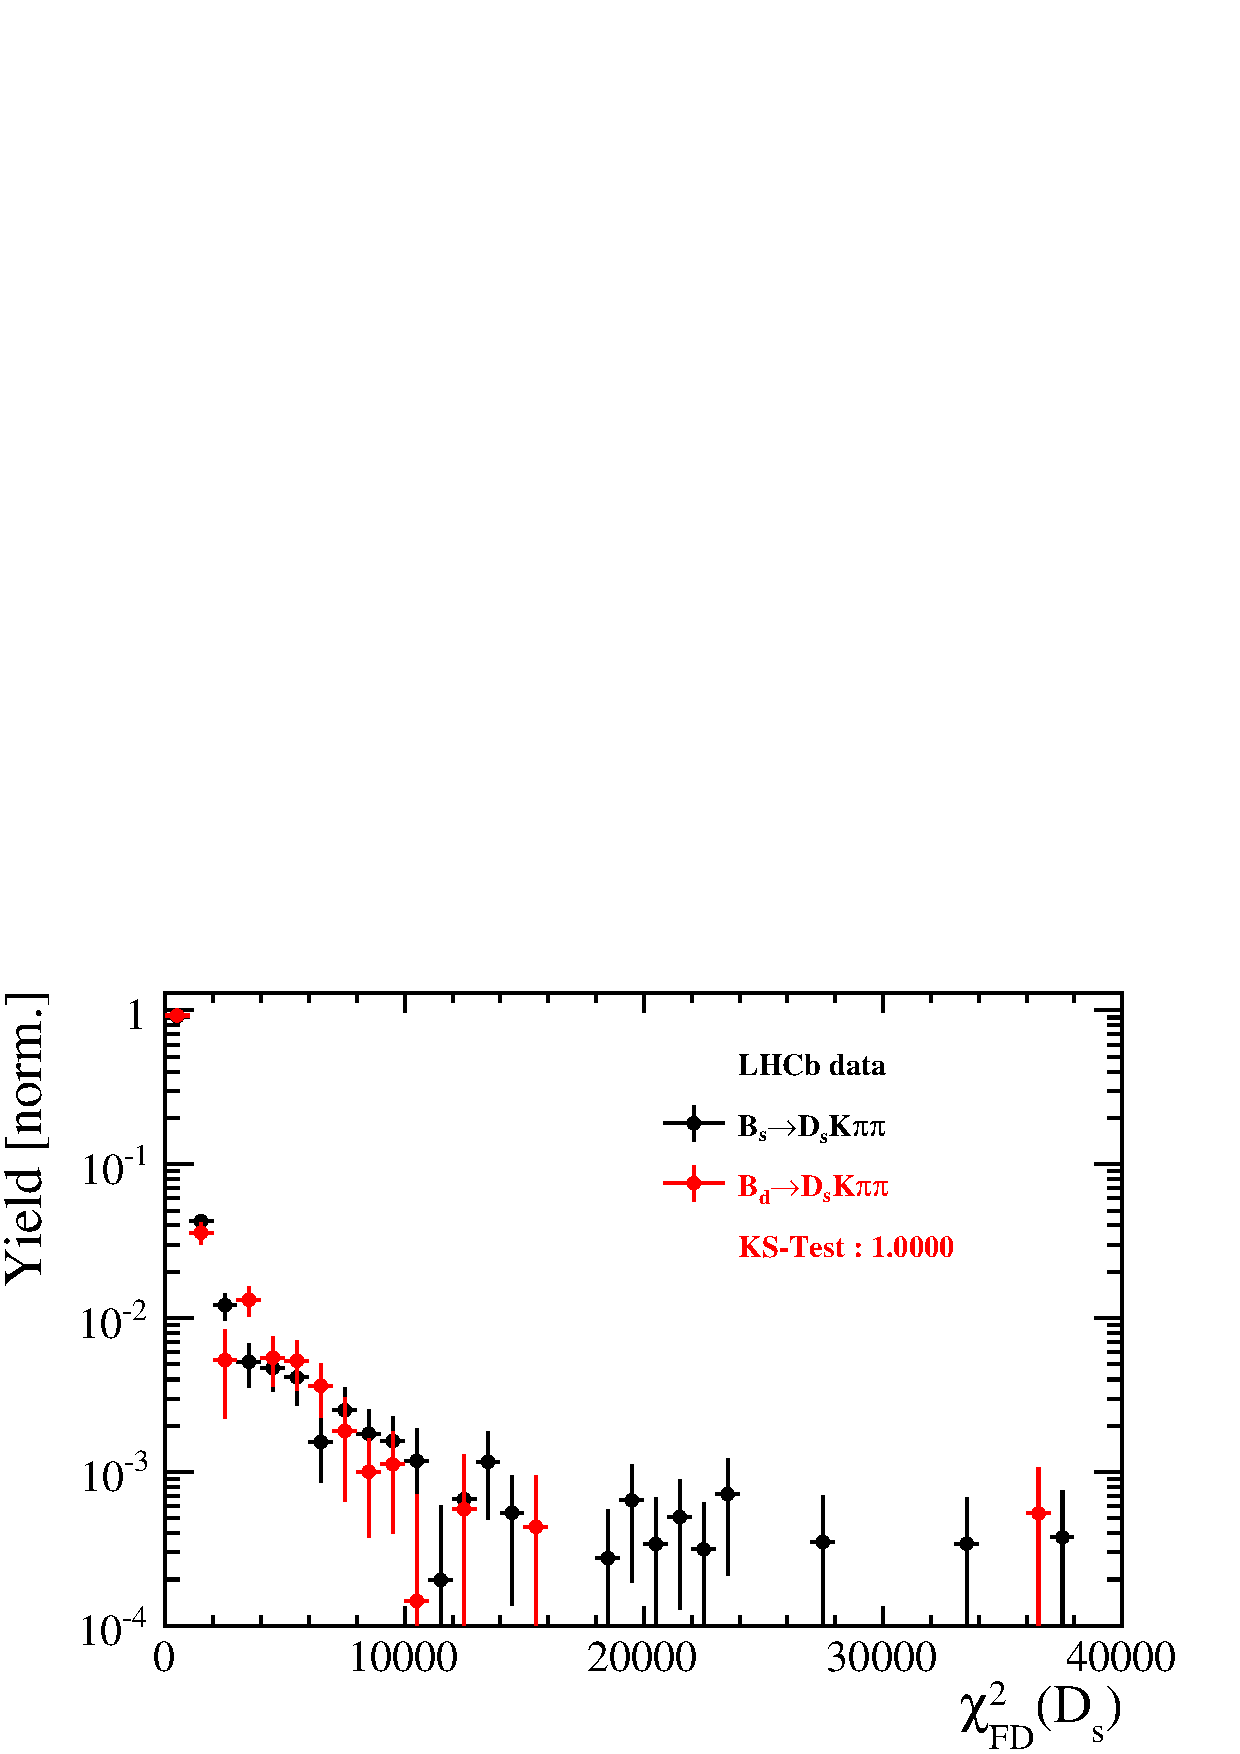
\includegraphics[height=!,width=0.4\textwidth]{figs/dataVsMC/norm2signal/Ds2all_Ds_FDCHI2_ORIVX.pdf}
%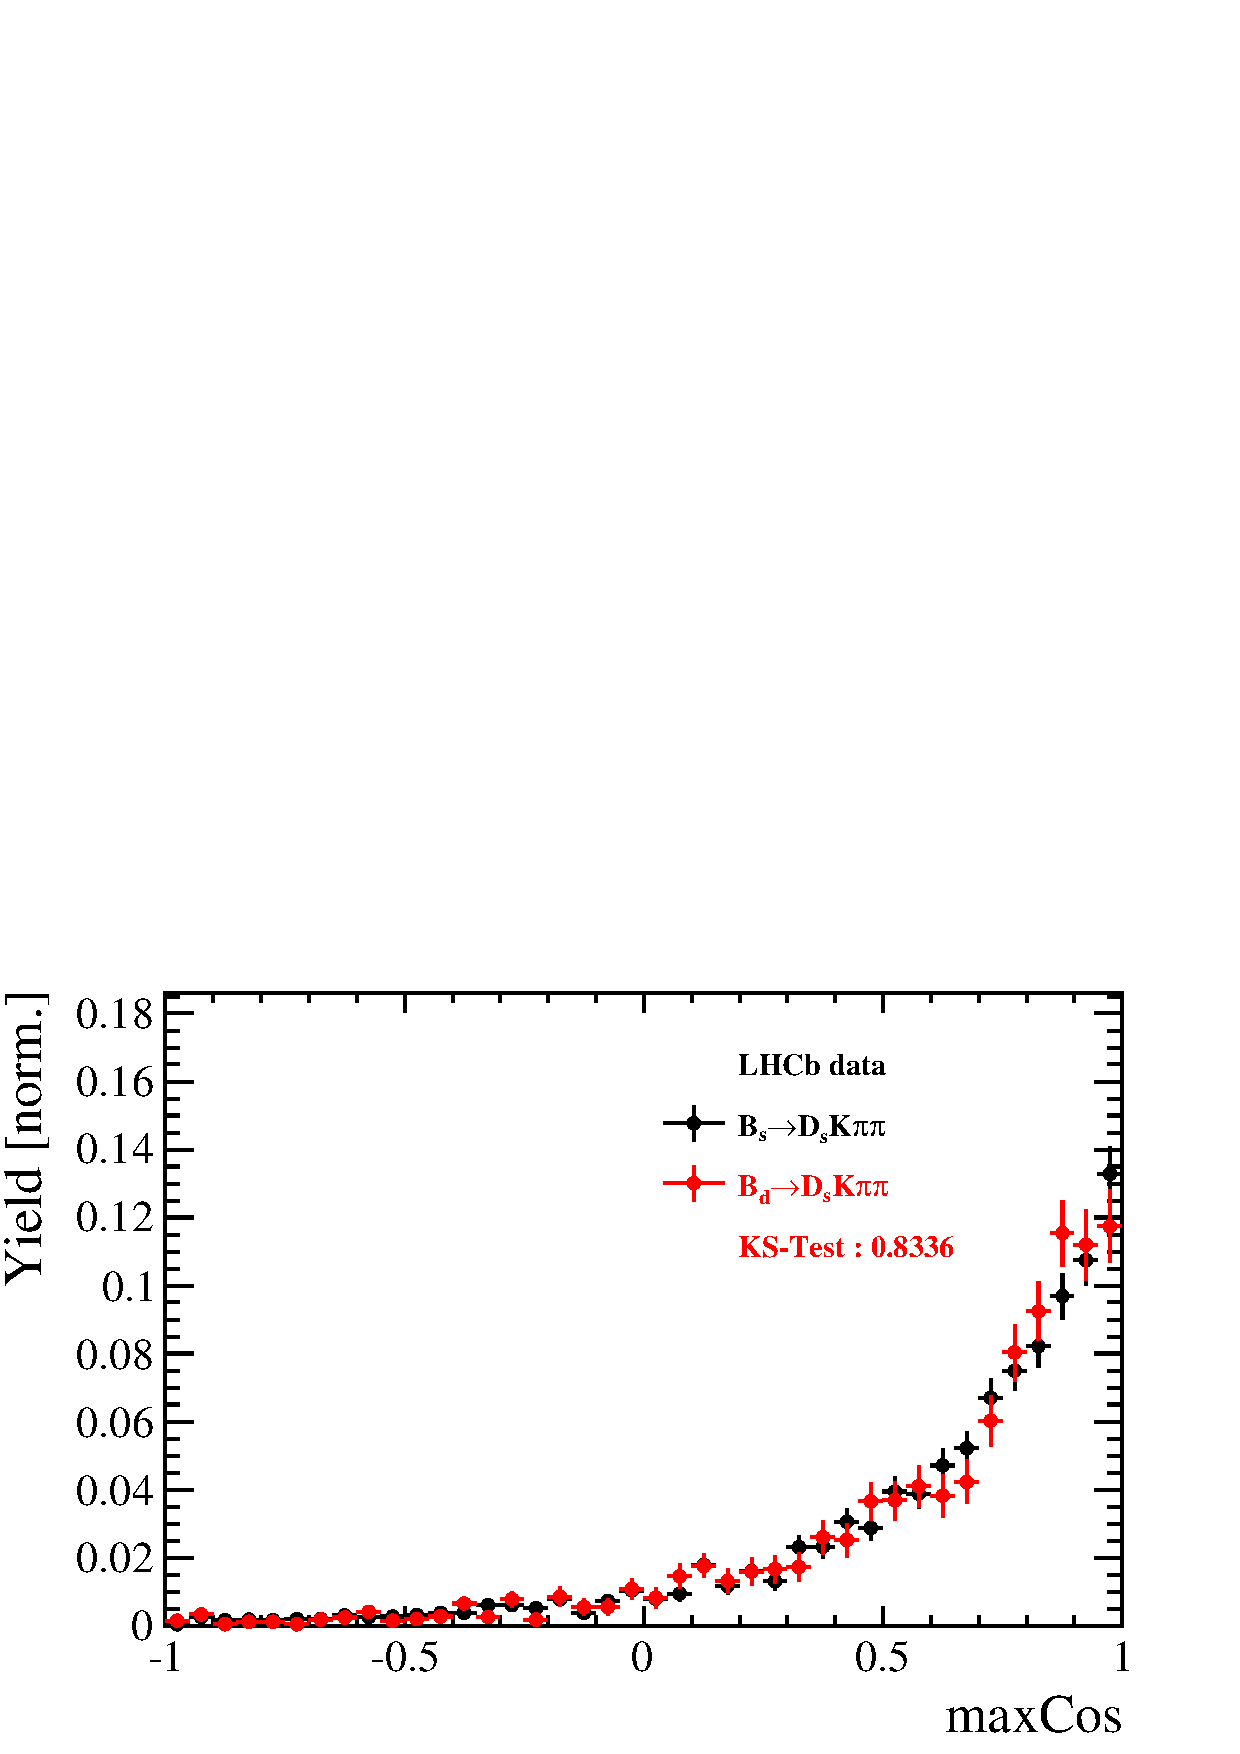
\includegraphics[height=!,width=0.4\textwidth]{figs/dataVsMC/norm2signal/Ds2all_maxCos.pdf}
%
%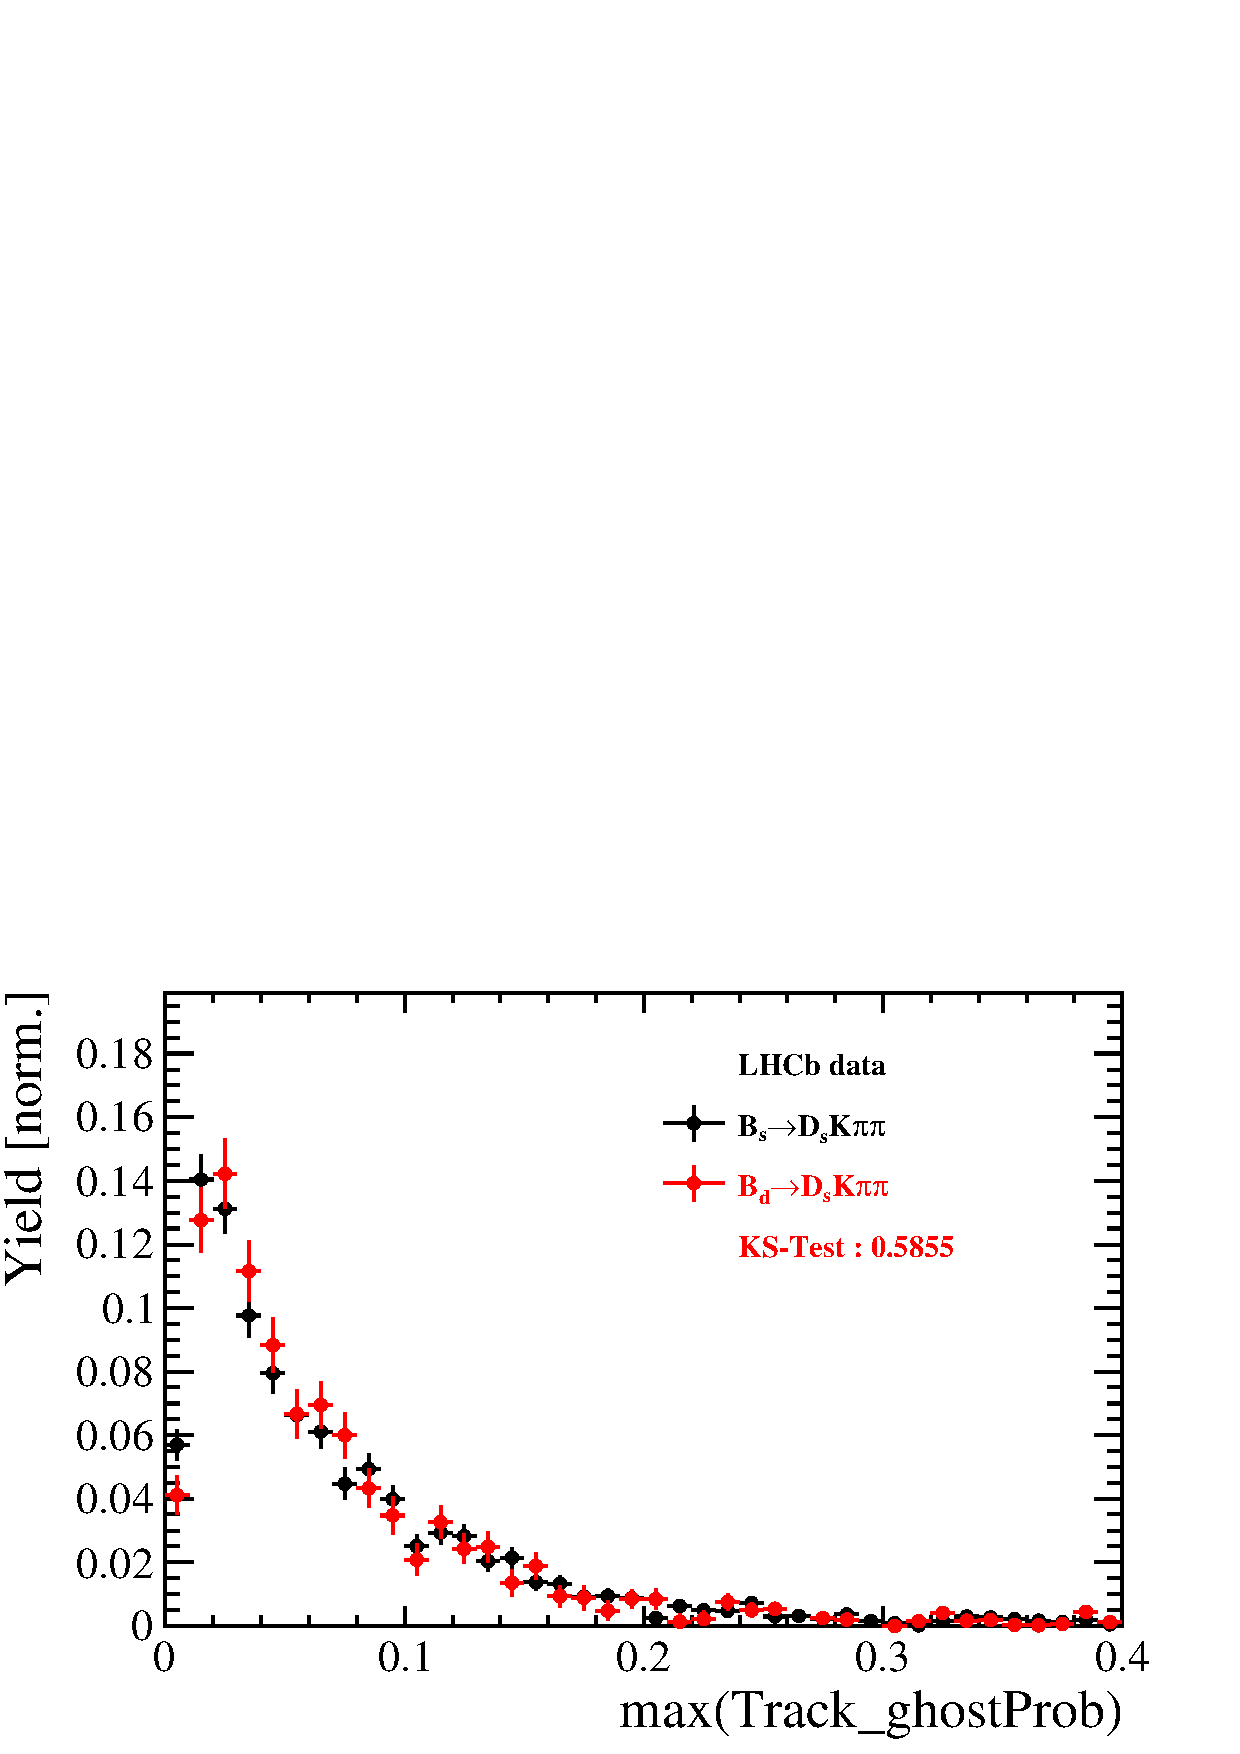
\includegraphics[height=!,width=0.4\textwidth]{figs/dataVsMC/norm2signal/Ds2all_max_ghostProb.pdf}
%%\includegraphics[height=!,width=0.5\textwidth]{figs/dataVsMC/norm_final/Ds2all_Bs_ptasy.00.pdf}
%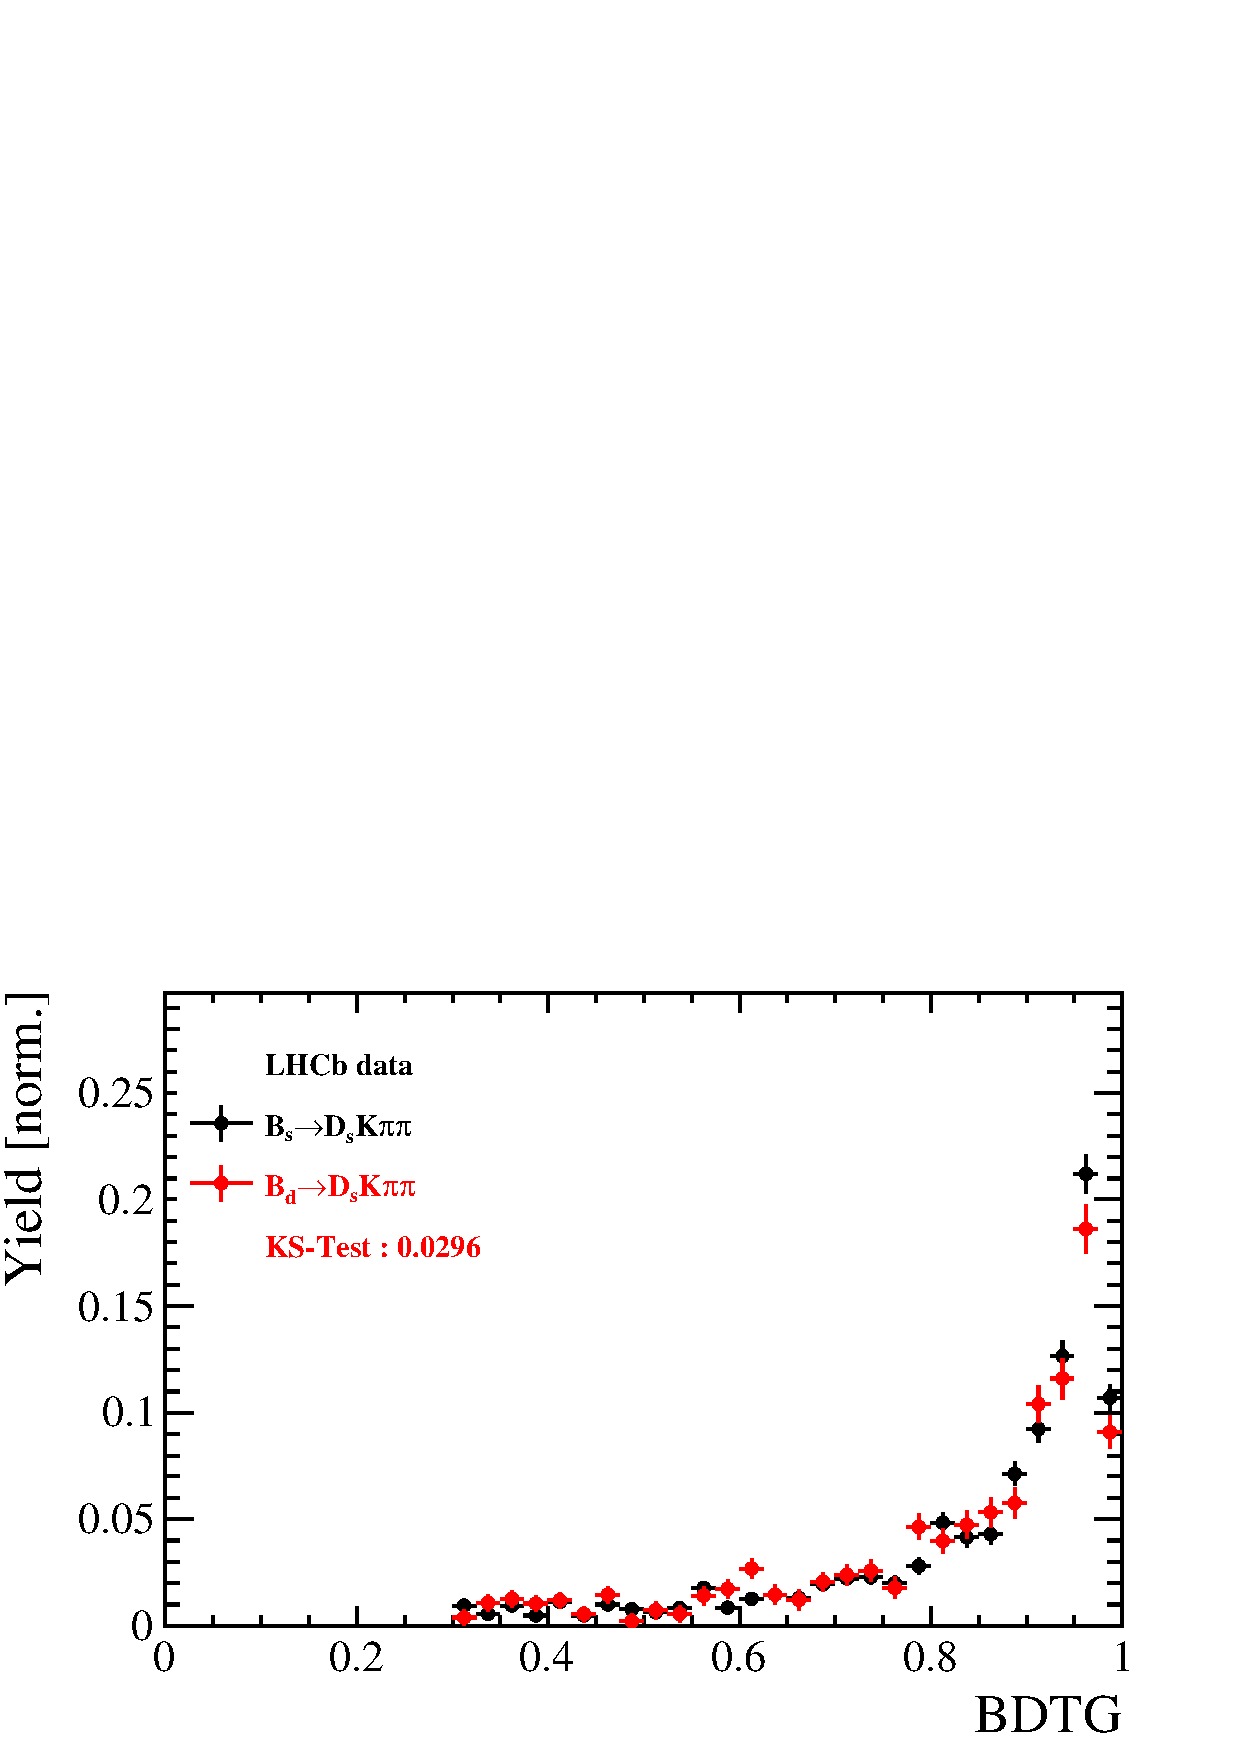
\includegraphics[height=!,width=0.4\textwidth]{figs/dataVsMC/norm2signal/Ds2all_BDTG_response.pdf}
%
%\caption{Comparison of BDTG input variables and classifier response.}
%\label{fig:}
%\end{figure}


\clearpage
\subsection*{Comparison of data taken in 2016 and 2017}
\label{ssec:16vs17}

\begin{figure}[h]
\centering
\includegraphics[height=!,width=0.3\textwidth]{figs/dataVsMC/year16vs17_norm/Ds2all_Bs_PT.pdf}
\includegraphics[height=!,width=0.3\textwidth]{figs/dataVsMC/year16vs17_norm/Ds2all_Bs_ETA.pdf}
\includegraphics[height=!,width=0.3\textwidth]{figs/dataVsMC/year16vs17_norm/Ds2all_NTracks.pdf}


\includegraphics[height=!,width=0.3\textwidth]{figs/dataVsMC/year16vs17_norm/Ds2all_Bs_BsDTF_TAUERR.pdf}
\includegraphics[height=!,width=0.3\textwidth]{figs/dataVsMC/year16vs17_norm/Ds2all_OS_Combination_PROB.pdf}
\includegraphics[height=!,width=0.3\textwidth]{figs/dataVsMC/year16vs17_norm/Ds2all_SS_Kaon_PROB.pdf}

\caption{Comparison of selected variables for $B_s \to D_s \pi \pi \pi$ data taken in 2016 and 2017.}
\label{fig:Norm_16v17}
\end{figure}

\begin{figure}[h]
\centering
\includegraphics[height=!,width=0.3\textwidth]{figs/dataVsMC/year16vs17_signal/Ds2all_Bs_DTF_MM.pdf}
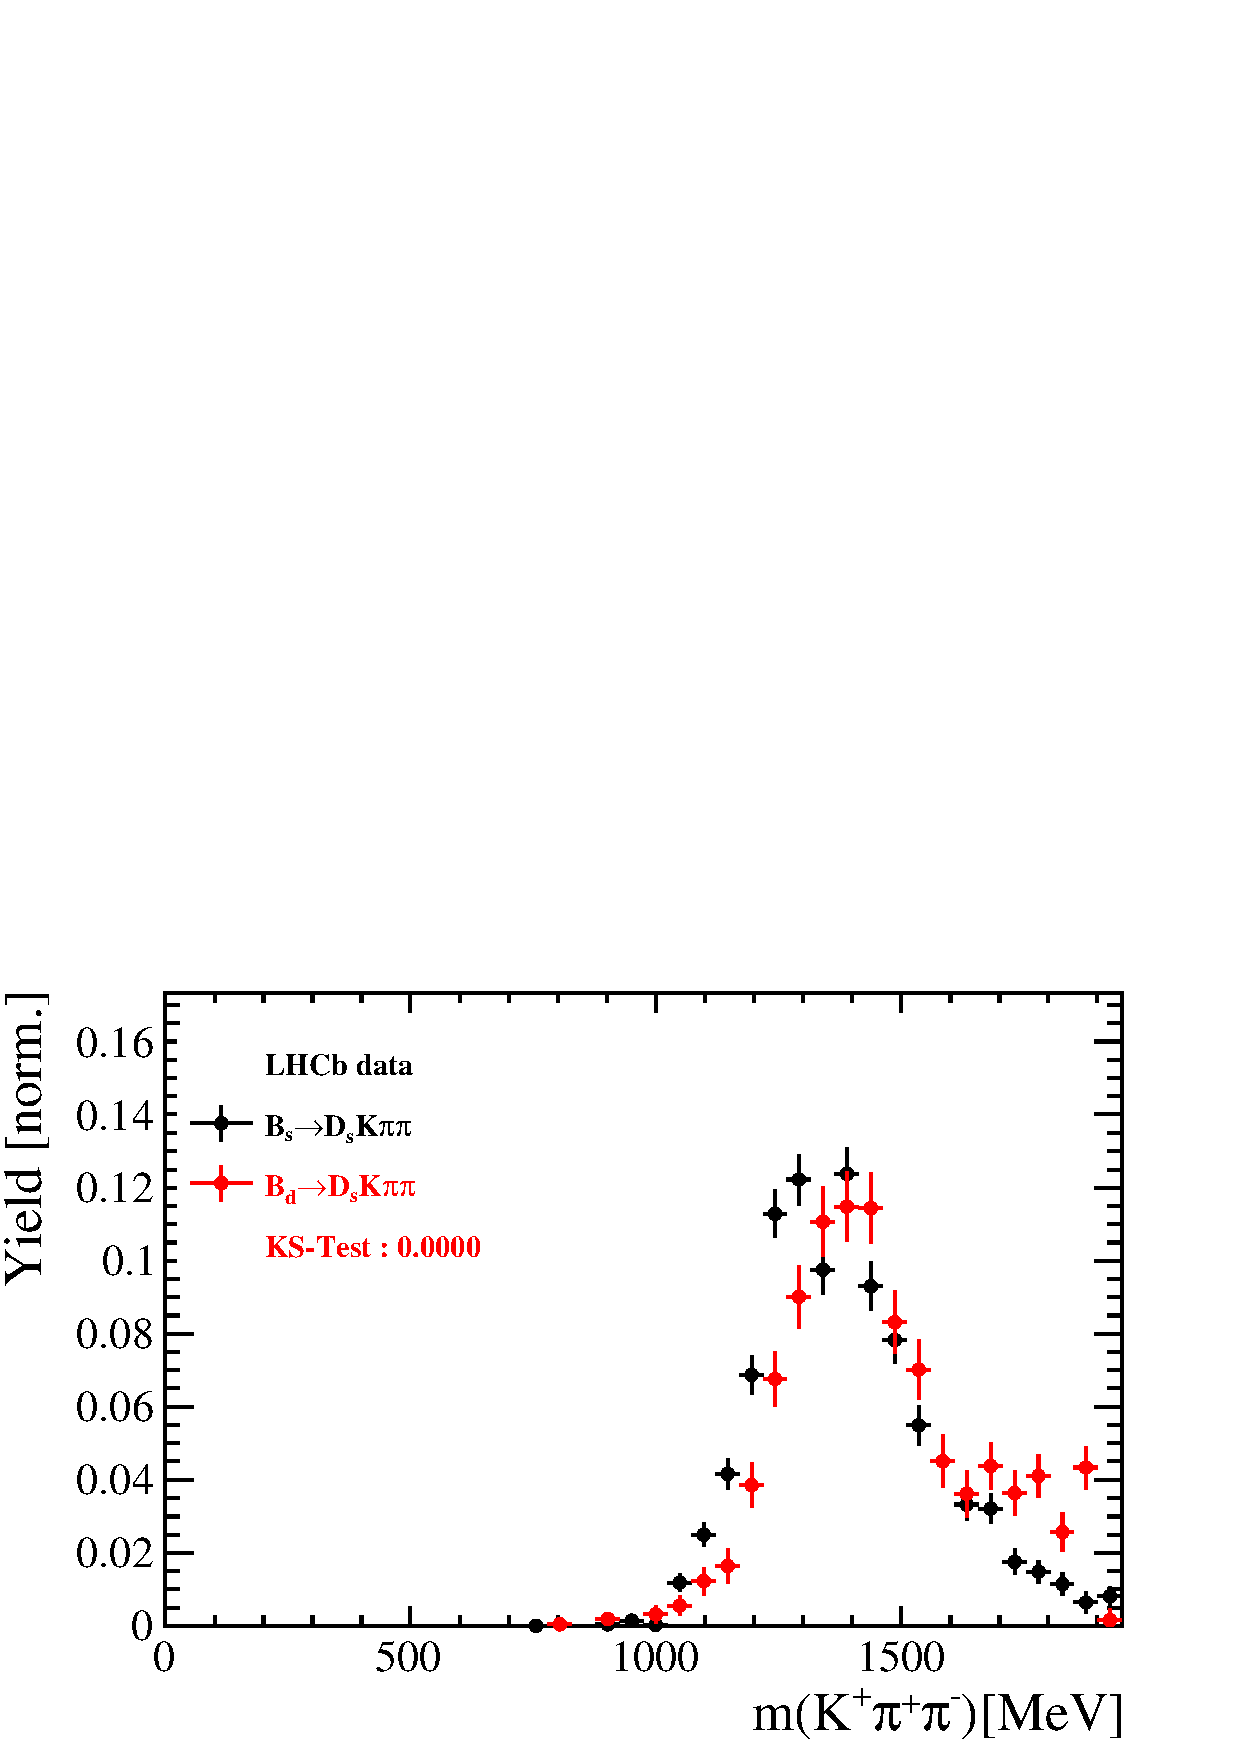
\includegraphics[height=!,width=0.3\textwidth]{figs/dataVsMC/year16vs17_signal/Ds2all_m_Kpipi.pdf}
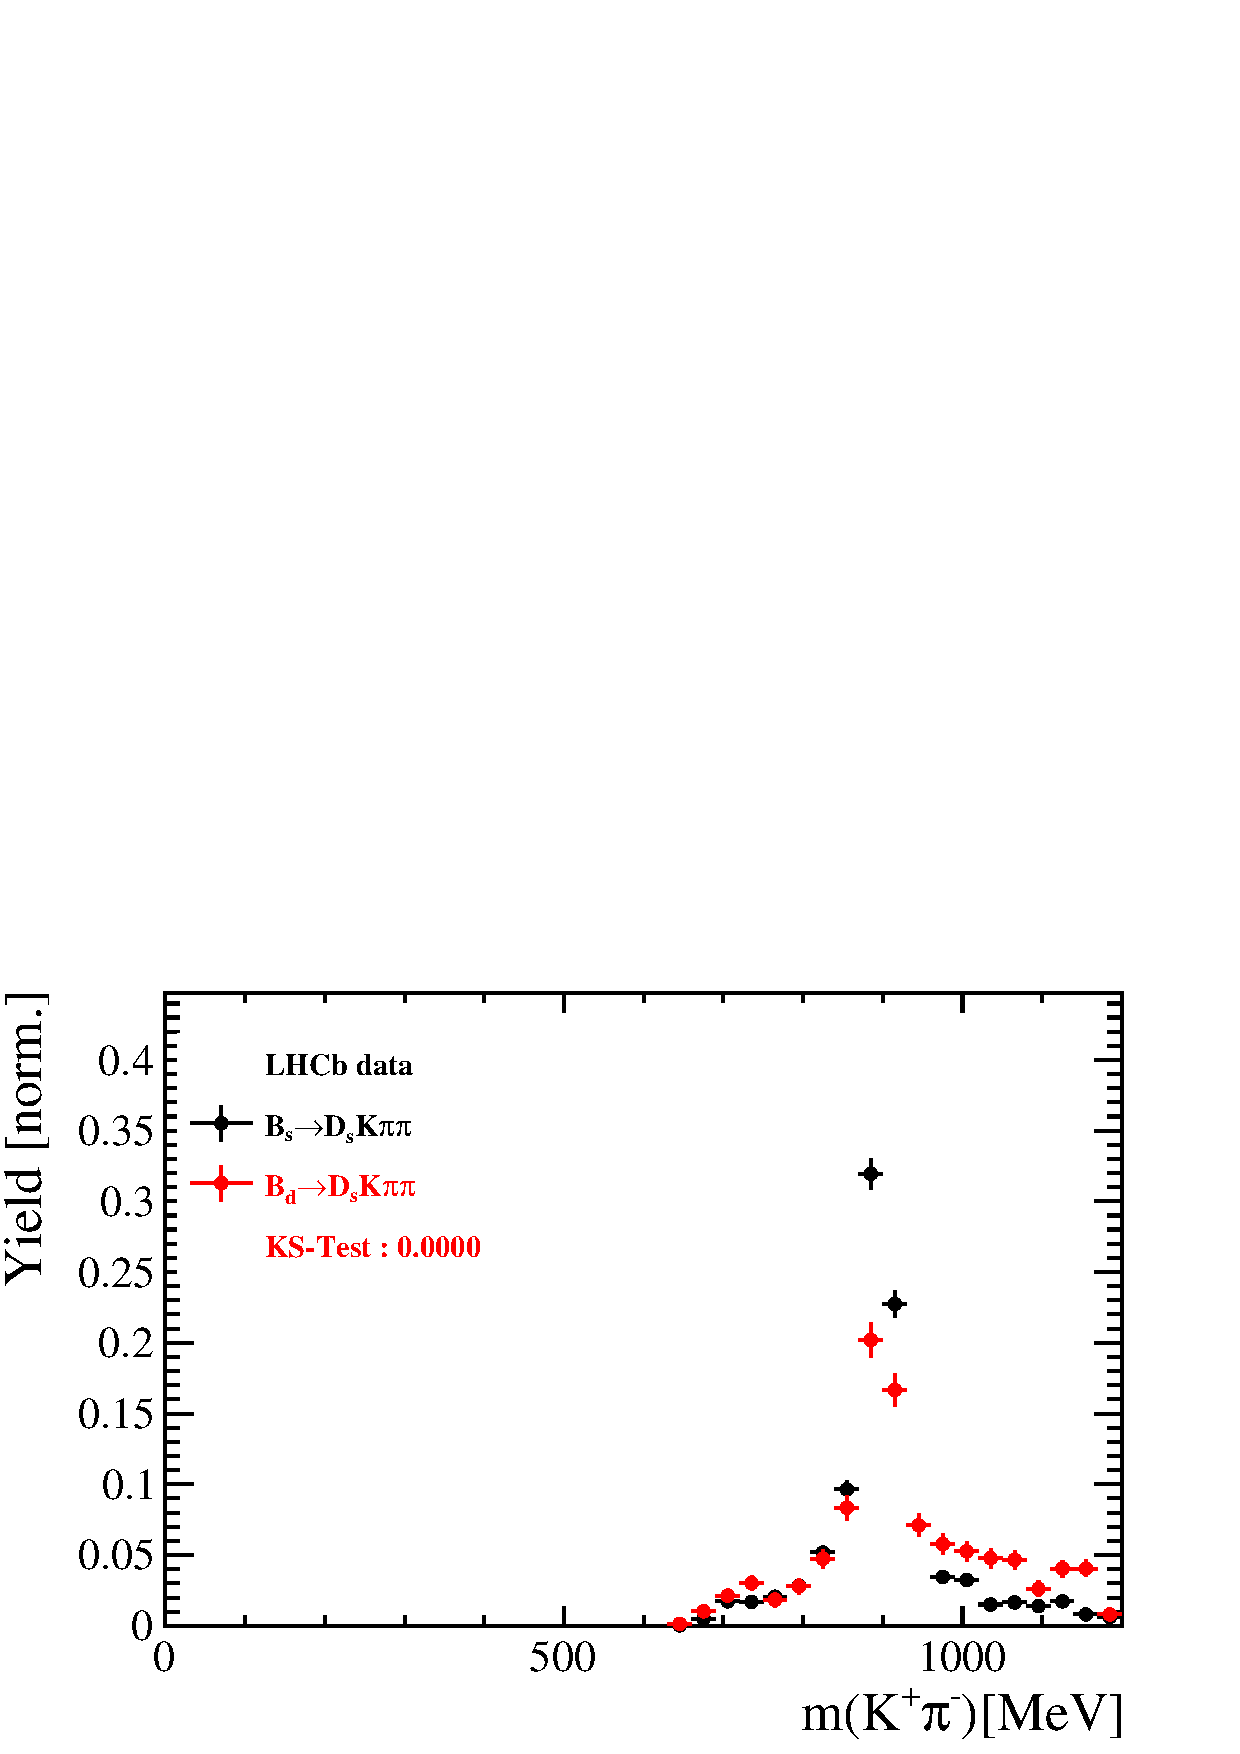
\includegraphics[height=!,width=0.3\textwidth]{figs/dataVsMC/year16vs17_signal/Ds2all_m_Kpi.pdf}

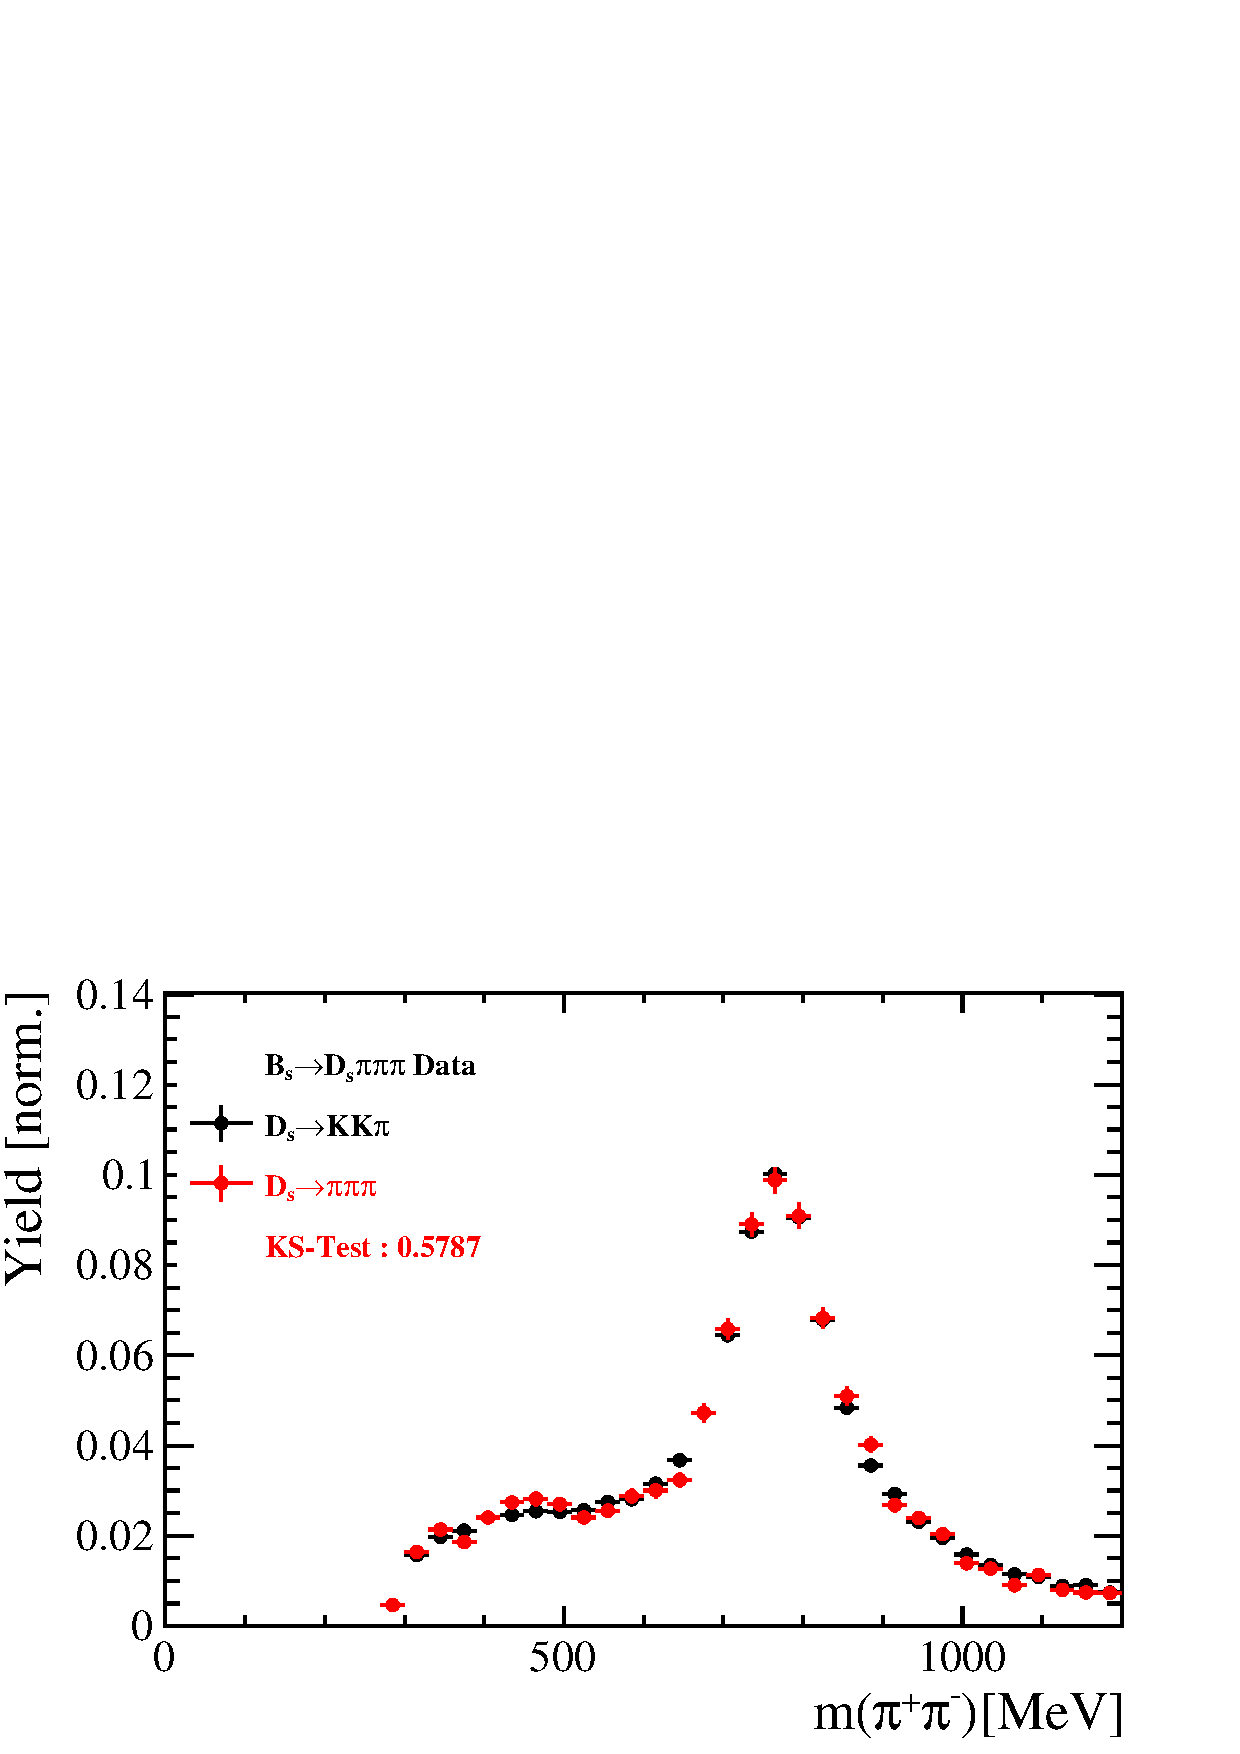
\includegraphics[height=!,width=0.3\textwidth]{figs/dataVsMC/year16vs17_signal/Ds2all_m_pipi.pdf}
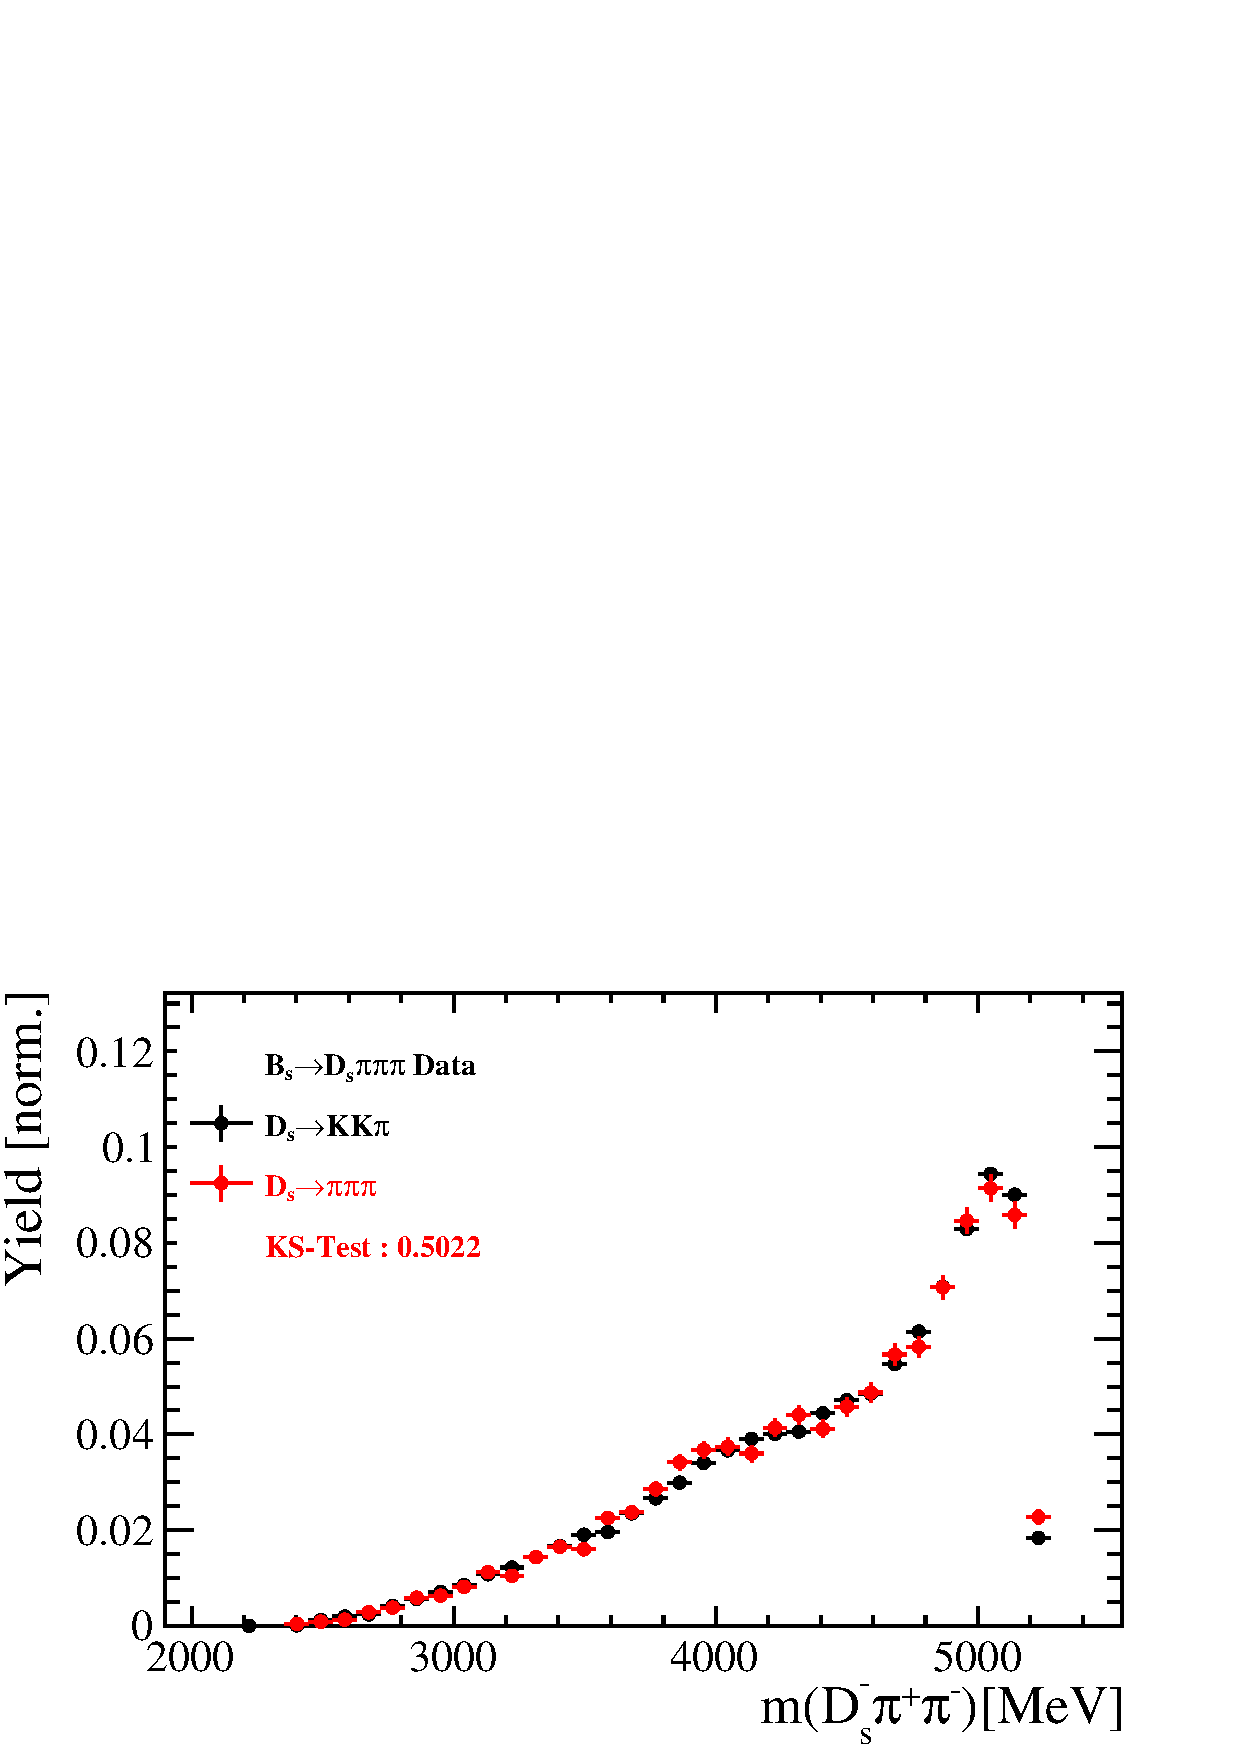
\includegraphics[height=!,width=0.3\textwidth]{figs/dataVsMC/year16vs17_signal/Ds2all_m_Dspipi.pdf}
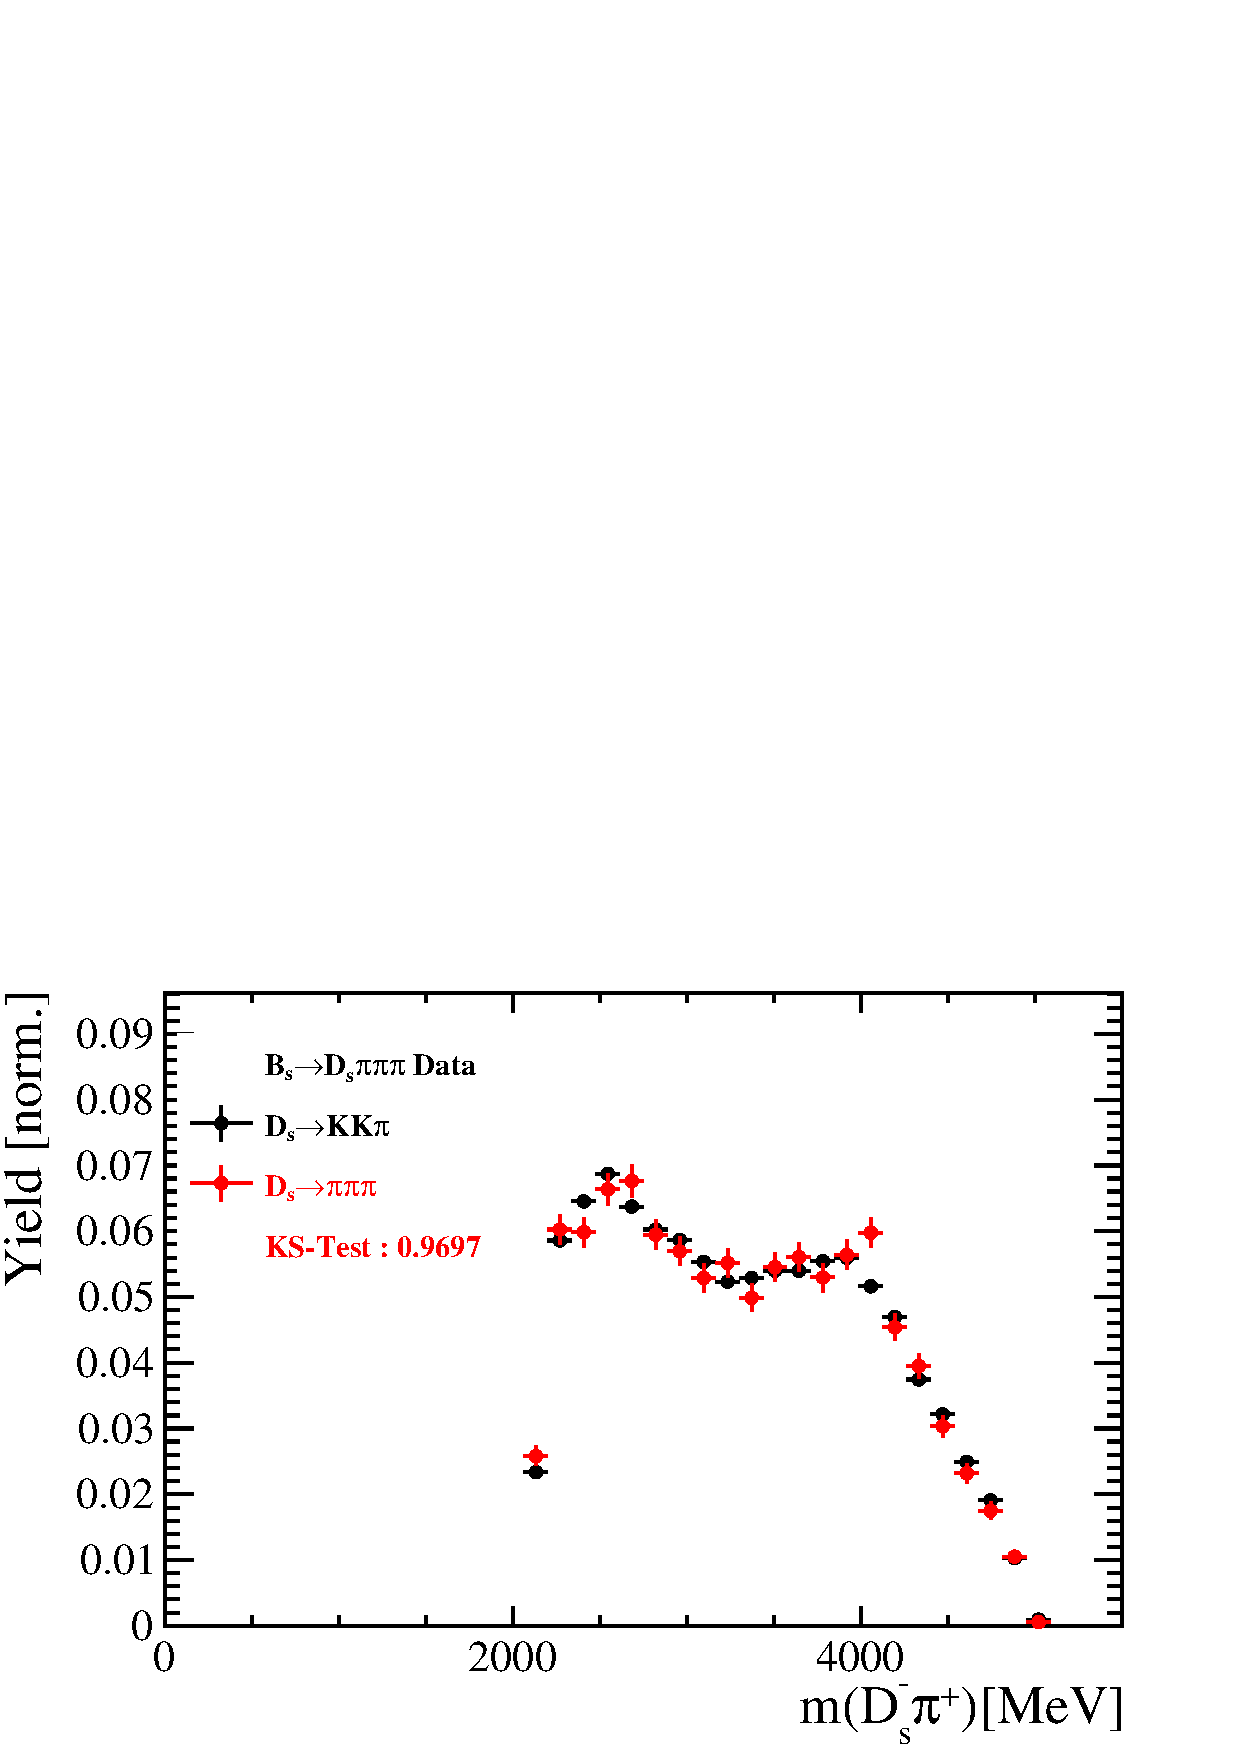
\includegraphics[height=!,width=0.3\textwidth]{figs/dataVsMC/year16vs17_signal/Ds2all_m_Dspi.pdf}

\caption{Comparison of selected variables for $B_s \to D_s K \pi \pi$ data taken in 2016 and 2017.}
\label{fig:}
\end{figure}


\clearpage
\subsection*{Comparison of Run-I and Run-II data}

\begin{figure}[h]
\centering
\includegraphics[height=!,width=0.3\textwidth]{figs/dataVsMC/run1vs2_norm/Ds2all_Bs_PT.pdf}
\includegraphics[height=!,width=0.3\textwidth]{figs/dataVsMC/run1vs2_norm/Ds2all_Bs_ETA.pdf}
\includegraphics[height=!,width=0.3\textwidth]{figs/dataVsMC/run1vs2_norm/Ds2all_NTracks.pdf}

%\includegraphics[height=!,width=0.4\textwidth]{figs/dataVsMC/run1vs2_norm/Ds2all_Bs_FDCHI2_OWNPV.pdf}
%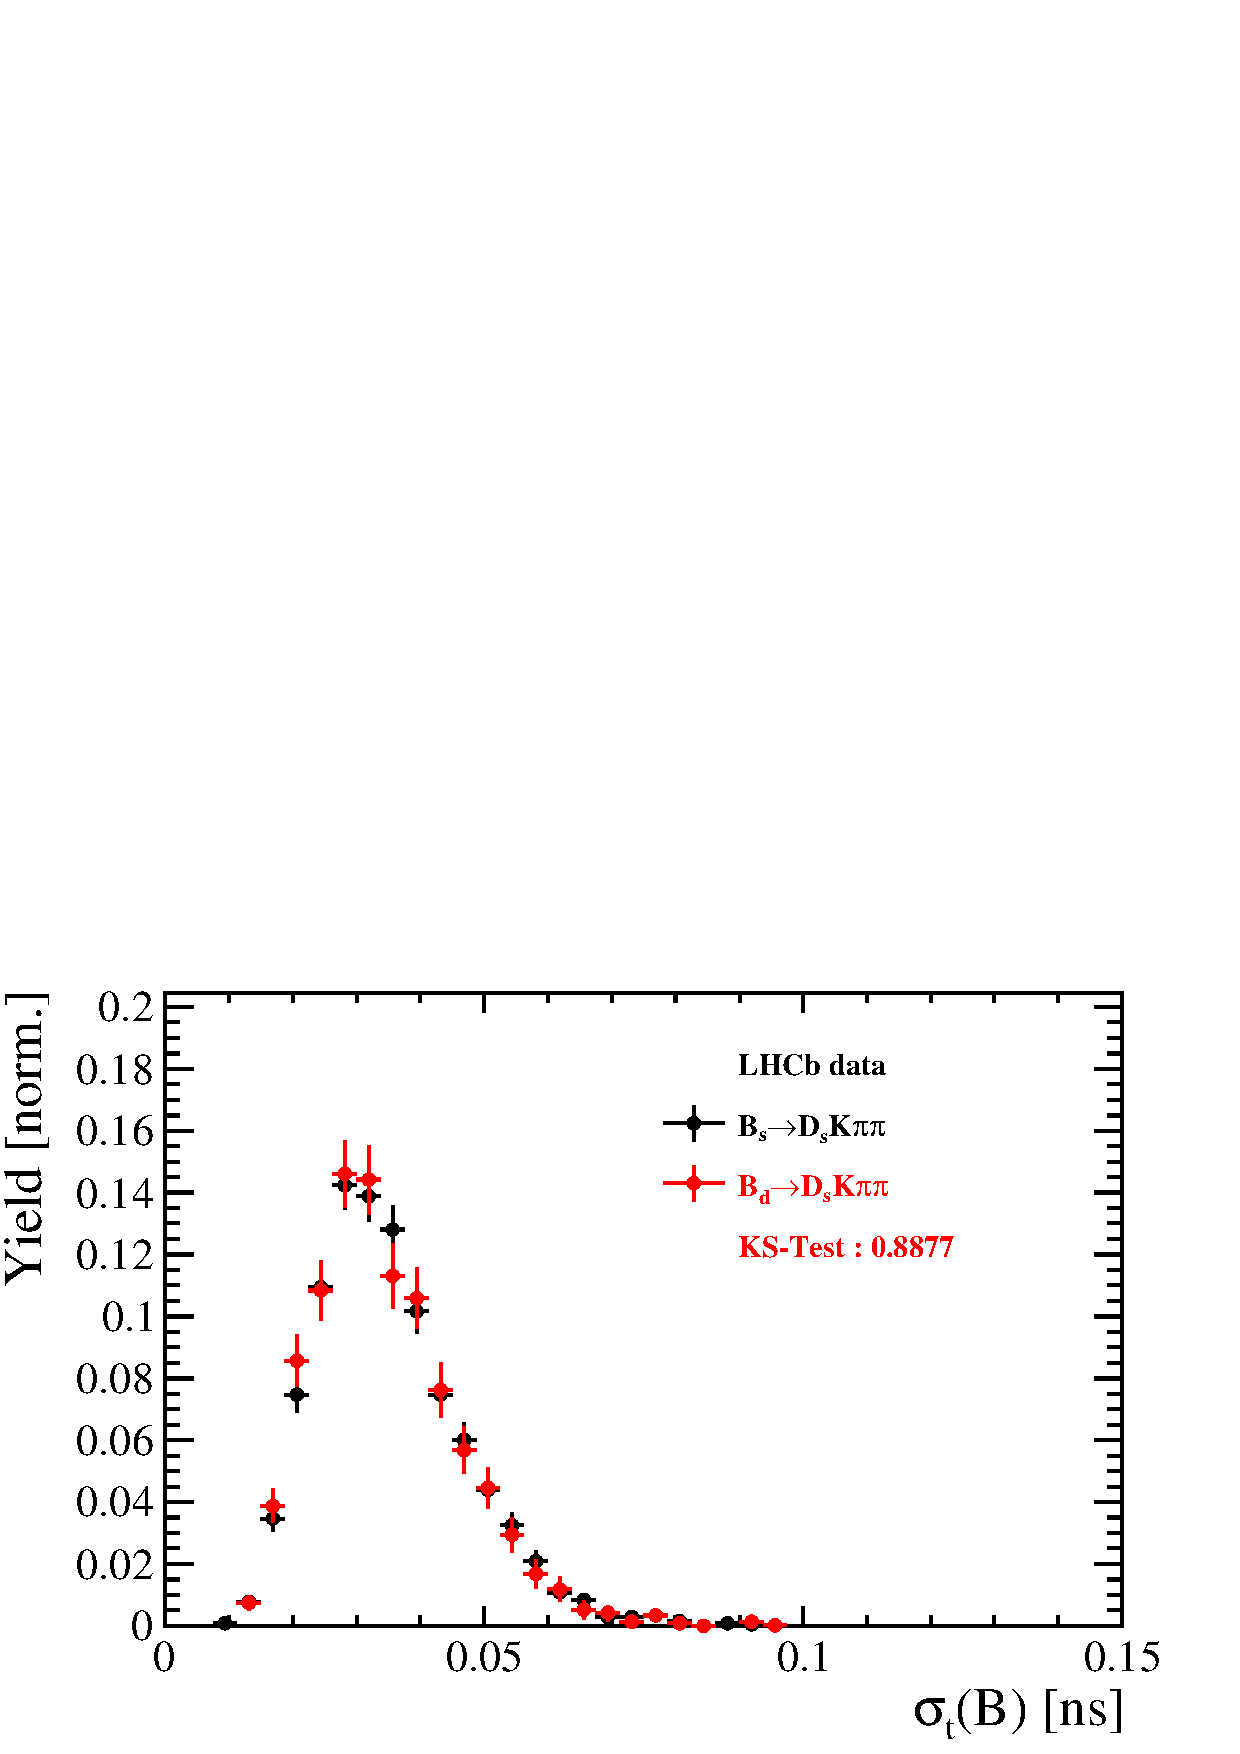
\includegraphics[height=!,width=0.4\textwidth]{figs/dataVsMC/run1vs2_norm/Ds2all_Bs_DTF_TAUERR.pdf}
%\includegraphics[height=!,width=0.4\textwidth]{figs/dataVsMC/run1vs2_norm/Ds2all_Bs_DTF_MERR.pdf}

\includegraphics[height=!,width=0.3\textwidth]{figs/dataVsMC/run1vs2_norm/Ds2all_Bs_BsDTF_TAUERR.pdf}
\includegraphics[height=!,width=0.3\textwidth]{figs/dataVsMC/run1vs2_norm/Ds2all_OS_Combination_PROB.pdf}
\includegraphics[height=!,width=0.3\textwidth]{figs/dataVsMC/run1vs2_norm/Ds2all_SS_Kaon_PROB.pdf}


\includegraphics[height=!,width=0.3\textwidth]{figs/dataVsMC/run1vs2_signal/Ds2all_Bs_DTF_MM.pdf}
\includegraphics[height=!,width=0.3\textwidth]{figs/dataVsMC/run1vs2_signal/Ds2all_m_Kpipi.pdf}
\includegraphics[height=!,width=0.3\textwidth]{figs/dataVsMC/run1vs2_signal/Ds2all_m_Kpi.pdf}

\includegraphics[height=!,width=0.3\textwidth]{figs/dataVsMC/run1vs2_signal/Ds2all_m_pipi.pdf}
\includegraphics[height=!,width=0.3\textwidth]{figs/dataVsMC/run1vs2_signal/Ds2all_m_Dspipi.pdf}
\includegraphics[height=!,width=0.3\textwidth]{figs/dataVsMC/run1vs2_signal/Ds2all_m_Dspi.pdf}

%\includegraphics[height=!,width=0.4\textwidth]{figs/dataVsMC/run1vs2_norm/Ds2all_Ds_m12.pdf}
%\includegraphics[height=!,width=0.4\textwidth]{figs/dataVsMC/run1vs2_norm/Ds2all_Ds_m13.pdf}

\caption{Comparison of selected variables for Run-I and Run-II data.}
\label{fig:}
\end{figure}

%\begin{figure}[h]
%\centering
%\includegraphics[height=!,width=0.4\textwidth]{figs/dataVsMC/run1vs2_norm/Ds2all_DTF_CHI2NDOF.pdf}
%\includegraphics[height=!,width=0.4\textwidth]{figs/dataVsMC/run1vs2_norm/Ds2all_Bs_IPCHI2_OWNPV.pdf}
%
%\includegraphics[height=!,width=0.4\textwidth]{figs/dataVsMC/run1vs2_norm/Ds2all_Bs_DIRA_OWNPV.pdf}
%\includegraphics[height=!,width=0.4\textwidth]{figs/dataVsMC/run1vs2_norm/Ds2all_XsDaughters_min_IPCHI2.pdf}
%
%\includegraphics[height=!,width=0.4\textwidth]{figs/dataVsMC/run1vs2_norm/Ds2all_Xs_max_DOCA.pdf}
%\includegraphics[height=!,width=0.4\textwidth]{figs/dataVsMC/run1vs2_norm/Ds2all_DsDaughters_min_IPCHI2.pdf}
%
%\includegraphics[height=!,width=0.4\textwidth]{figs/dataVsMC/run1vs2_norm/Ds2all_Ds_FDCHI2_ORIVX.pdf}
%\includegraphics[height=!,width=0.4\textwidth]{figs/dataVsMC/run1vs2_norm/Ds2all_maxCos.pdf}
%
%\includegraphics[height=!,width=0.4\textwidth]{figs/dataVsMC/run1vs2_norm/Ds2all_max_ghostProb.pdf}
%%\includegraphics[height=!,width=0.5\textwidth]{figs/dataVsMC/run1vs2_norm/Ds2all_Bs_ptasy.00.pdf}
%\includegraphics[height=!,width=0.4\textwidth]{figs/dataVsMC/run1vs2_norm/Ds2all_BDTG_response.pdf}
%
%\caption{Comparison of BDTG input variables and classifier response.}
%\label{fig:}
%\end{figure}



\clearpage
\subsection*{Comparison of $D_s$ final states}

\begin{figure}[h]
\centering
\includegraphics[height=!,width=0.3\textwidth]{figs/dataVsMC/finalState_norm/Ds2all_Bs_PT.pdf}
\includegraphics[height=!,width=0.3\textwidth]{figs/dataVsMC/finalState_norm/Ds2all_Bs_ETA.pdf}
\includegraphics[height=!,width=0.3\textwidth]{figs/dataVsMC/finalState_norm/Ds2all_NTracks.pdf}

%\includegraphics[height=!,width=0.4\textwidth]{figs/dataVsMC/finalState_norm/Ds2all_Bs_FDCHI2_OWNPV.pdf}
%\includegraphics[height=!,width=0.4\textwidth]{figs/dataVsMC/finalState_norm/Ds2all_Bs_DTF_MERR.pdf}

\includegraphics[height=!,width=0.3\textwidth]{figs/dataVsMC/finalState_norm/Ds2all_Bs_BsDTF_TAUERR.pdf}
\includegraphics[height=!,width=0.3\textwidth]{figs/dataVsMC/finalState_norm/Ds2all_OS_Combination_PROB.pdf}
\includegraphics[height=!,width=0.3\textwidth]{figs/dataVsMC/finalState_norm/Ds2all_SS_Kaon_PROB.pdf}

%\includegraphics[height=!,width=0.4\textwidth]{figs/dataVsMC/finalState_norm/Ds2all_Ds_m12.pdf}
%\includegraphics[height=!,width=0.4\textwidth]{figs/dataVsMC/finalState_norm/Ds2all_Ds_m13.pdf}

\includegraphics[height=!,width=0.3\textwidth]{figs/dataVsMC/finalState_signal/Ds2all_Bs_DTF_MM.pdf}
\includegraphics[height=!,width=0.3\textwidth]{figs/dataVsMC/finalState_signal/Ds2all_m_Kpipi.pdf}
\includegraphics[height=!,width=0.3\textwidth]{figs/dataVsMC/finalState_signal/Ds2all_m_Kpi.pdf}

\includegraphics[height=!,width=0.3\textwidth]{figs/dataVsMC/finalState_signal/Ds2all_m_pipi.pdf}
\includegraphics[height=!,width=0.3\textwidth]{figs/dataVsMC/finalState_signal/Ds2all_m_Dspipi.pdf}
\includegraphics[height=!,width=0.3\textwidth]{figs/dataVsMC/finalState_signal/Ds2all_m_Dspi.pdf}

\caption{Comparison of selected variables for different $D_s$ final states.}
\label{fig:}
\end{figure}


\begin{figure}[h]
\centering
\includegraphics[height=!,width=0.3\textwidth]{figs/dataVsMC/finalState2_norm/Ds2all_Bs_PT.pdf}
\includegraphics[height=!,width=0.3\textwidth]{figs/dataVsMC/finalState2_norm/Ds2all_Bs_ETA.pdf}
\includegraphics[height=!,width=0.3\textwidth]{figs/dataVsMC/finalState2_norm/Ds2all_NTracks.pdf}

\includegraphics[height=!,width=0.3\textwidth]{figs/dataVsMC/finalState2_norm/Ds2all_Bs_BsDTF_TAUERR.pdf}
\includegraphics[height=!,width=0.3\textwidth]{figs/dataVsMC/finalState2_norm/Ds2all_OS_Combination_PROB.pdf}
\includegraphics[height=!,width=0.3\textwidth]{figs/dataVsMC/finalState2_norm/Ds2all_SS_Kaon_PROB.pdf}

\includegraphics[height=!,width=0.3\textwidth]{figs/dataVsMC/finalState2_signal/Ds2all_Bs_DTF_MM.pdf}
\includegraphics[height=!,width=0.3\textwidth]{figs/dataVsMC/finalState2_signal/Ds2all_m_Kpipi.pdf}
\includegraphics[height=!,width=0.3\textwidth]{figs/dataVsMC/finalState2_signal/Ds2all_m_Kpi.pdf}

\includegraphics[height=!,width=0.3\textwidth]{figs/dataVsMC/finalState2_signal/Ds2all_m_pipi.pdf}
\includegraphics[height=!,width=0.3\textwidth]{figs/dataVsMC/finalState2_signal/Ds2all_m_Dspipi.pdf}
\includegraphics[height=!,width=0.3\textwidth]{figs/dataVsMC/finalState2_signal/Ds2all_m_Dspi.pdf}

\caption{Comparison of selected variables for different $D_s$ final states.}
\label{fig:}
\end{figure}

%\begin{figure}[h]
%\centering
%\includegraphics[height=!,width=0.4\textwidth]{figs/dataVsMC/finalState_norm/Ds2all_DTF_CHI2NDOF.pdf}
%\includegraphics[height=!,width=0.4\textwidth]{figs/dataVsMC/finalState_norm/Ds2all_Bs_IPCHI2_OWNPV.pdf}
%
%\includegraphics[height=!,width=0.4\textwidth]{figs/dataVsMC/finalState_norm/Ds2all_Bs_DIRA_OWNPV.pdf}
%\includegraphics[height=!,width=0.4\textwidth]{figs/dataVsMC/finalState_norm/Ds2all_XsDaughters_min_IPCHI2.pdf}
%
%\includegraphics[height=!,width=0.4\textwidth]{figs/dataVsMC/finalState_norm/Ds2all_Xs_max_DOCA.pdf}
%\includegraphics[height=!,width=0.4\textwidth]{figs/dataVsMC/finalState_norm/Ds2all_DsDaughters_min_IPCHI2.pdf}
%
%\includegraphics[height=!,width=0.4\textwidth]{figs/dataVsMC/finalState_norm/Ds2all_Ds_FDCHI2_ORIVX.pdf}
%\includegraphics[height=!,width=0.4\textwidth]{figs/dataVsMC/finalState_norm/Ds2all_maxCos.pdf}
%
%\includegraphics[height=!,width=0.4\textwidth]{figs/dataVsMC/finalState_norm/Ds2all_max_ghostProb.pdf}
%%\includegraphics[height=!,width=0.5\textwidth]{figs/dataVsMC/finalState_norm/Ds2all_Bs_ptasy.00.pdf}
%\includegraphics[height=!,width=0.4\textwidth]{figs/dataVsMC/finalState_norm/Ds2all_BDTG_response.pdf}
%
%\caption{Comparison of BDTG input variables and classifier response.}
%\label{fig:}
%\end{figure}

\clearpage
\subsection*{Comparison of trigger categories}

\begin{figure}[h]
\centering
\includegraphics[height=!,width=0.3\textwidth]{figs/dataVsMC/trigger_norm/Ds2all_Bs_PT.pdf}
\includegraphics[height=!,width=0.3\textwidth]{figs/dataVsMC/trigger_norm/Ds2all_Bs_ETA.pdf}
\includegraphics[height=!,width=0.3\textwidth]{figs/dataVsMC/trigger_norm/Ds2all_NTracks.pdf}

\includegraphics[height=!,width=0.3\textwidth]{figs/dataVsMC/trigger_norm/Ds2all_Bs_BsDTF_TAUERR.pdf}
\includegraphics[height=!,width=0.3\textwidth]{figs/dataVsMC/trigger_norm/Ds2all_OS_Combination_PROB.pdf}
\includegraphics[height=!,width=0.3\textwidth]{figs/dataVsMC/trigger_norm/Ds2all_SS_Kaon_PROB.pdf}

\includegraphics[height=!,width=0.3\textwidth]{figs/dataVsMC/trigger_signal/Ds2all_Bs_DTF_MM.pdf}
\includegraphics[height=!,width=0.3\textwidth]{figs/dataVsMC/trigger_signal/Ds2all_m_Kpipi.pdf}
\includegraphics[height=!,width=0.3\textwidth]{figs/dataVsMC/trigger_signal/Ds2all_m_Kpi.pdf}

\includegraphics[height=!,width=0.3\textwidth]{figs/dataVsMC/trigger_signal/Ds2all_m_pipi.pdf}
\includegraphics[height=!,width=0.3\textwidth]{figs/dataVsMC/trigger_signal/Ds2all_m_Dspipi.pdf}
\includegraphics[height=!,width=0.3\textwidth]{figs/dataVsMC/trigger_signal/Ds2all_m_Dspi.pdf}

\caption{Comparison of selected variables for different trigger categories.}
\label{fig:}
\end{figure}

%\begin{figure}[h]
%\centering
%\includegraphics[height=!,width=0.4\textwidth]{figs/dataVsMC/trigger_norm/Ds2all_DTF_CHI2NDOF.pdf}
%\includegraphics[height=!,width=0.4\textwidth]{figs/dataVsMC/trigger_norm/Ds2all_Bs_IPCHI2_OWNPV.pdf}
%
%\includegraphics[height=!,width=0.4\textwidth]{figs/dataVsMC/trigger_norm/Ds2all_Bs_DIRA_OWNPV.pdf}
%\includegraphics[height=!,width=0.4\textwidth]{figs/dataVsMC/trigger_norm/Ds2all_XsDaughters_min_IPCHI2.pdf}
%
%\includegraphics[height=!,width=0.4\textwidth]{figs/dataVsMC/trigger_norm/Ds2all_Xs_max_DOCA.pdf}
%\includegraphics[height=!,width=0.4\textwidth]{figs/dataVsMC/trigger_norm/Ds2all_DsDaughters_min_IPCHI2.pdf}
%
%\includegraphics[height=!,width=0.4\textwidth]{figs/dataVsMC/trigger_norm/Ds2all_Ds_FDCHI2_ORIVX.pdf}
%\includegraphics[height=!,width=0.4\textwidth]{figs/dataVsMC/trigger_norm/Ds2all_maxCos.pdf}
%
%\includegraphics[height=!,width=0.4\textwidth]{figs/dataVsMC/trigger_norm/Ds2all_max_ghostProb.pdf}
%%\includegraphics[height=!,width=0.5\textwidth]{figs/dataVsMC/trigger_norm/Ds2all_Bs_ptasy.00.pdf}
%\includegraphics[height=!,width=0.4\textwidth]{figs/dataVsMC/trigger_norm/Ds2all_BDTG_response.pdf}
%
%\caption{Comparison of BDTG input variables and classifier response.}
%\label{fig:}
%\end{figure}


%\clearpage
%\subsection{Comparison of $B_s$ and $B_d$ decays}
%
%\begin{figure}[h]
%\centering
%\includegraphics[height=!,width=0.3\textwidth]{figs/dataVsMC/B0vsBs_signal/Ds2all_Bs_PT.pdf}
%\includegraphics[height=!,width=0.3\textwidth]{figs/dataVsMC/B0vsBs_signal/Ds2all_Bs_ETA.pdf}
%\includegraphics[height=!,width=0.3\textwidth]{figs/dataVsMC/B0vsBs_signal/Ds2all_NTracks.pdf}
%
%%\includegraphics[height=!,width=0.4\textwidth]{figs/dataVsMC/B0vsBs_signal/Ds2all_Bs_FDCHI2_OWNPV.pdf}
%%\includegraphics[height=!,width=0.4\textwidth]{figs/dataVsMC/B0vsBs_signal/Ds2all_Bs_IPCHI2_OWNPV.pdf}
%%\includegraphics[height=!,width=0.4\textwidth]{figs/dataVsMC/B0vsBs_signal/Ds2all_Bs_DIRA_OWNPV.pdf}
%
%%\includegraphics[height=!,width=0.3\textwidth]{figs/dataVsMC/B0vsBs_signal/Ds2all_Bs_DTF_TAUERR.pdf}
%%%\includegraphics[height=!,width=0.4\textwidth]{figs/dataVsMC/B0vsBs_signal/Ds2all_Bs_DTF_MERR.pdf}
%%\includegraphics[height=!,width=0.3\textwidth]{figs/dataVsMC/B0vsBs_signal/Ds2all_Bs_TAGOMEGA_OS.pdf}
%%\includegraphics[height=!,width=0.3\textwidth]{figs/dataVsMC/B0vsBs_signal/Ds2all_Bs_SS_nnetKaon_PROB.pdf}
%
%%\includegraphics[height=!,width=0.4\textwidth]{figs/dataVsMC/B0vsBs_signal/Ds2all_Ds_m12.pdf}
%%\includegraphics[height=!,width=0.4\textwidth]{figs/dataVsMC/B0vsBs_signal/Ds2all_Ds_m13.pdf}
%
%\caption{Comparison of selected variables.}
%\label{fig:}
%\end{figure}
%
%%\begin{figure}[h]
%%\centering
%%\includegraphics[height=!,width=0.4\textwidth]{figs/dataVsMC/B0vsBs_signal/Ds2all_DTF_CHI2NDOF.pdf}
%%\includegraphics[height=!,width=0.4\textwidth]{figs/dataVsMC/B0vsBs_signal/Ds2all_Bs_IPCHI2_OWNPV.pdf}
%%
%%\includegraphics[height=!,width=0.4\textwidth]{figs/dataVsMC/B0vsBs_signal/Ds2all_Bs_DIRA_OWNPV.pdf}
%%\includegraphics[height=!,width=0.4\textwidth]{figs/dataVsMC/B0vsBs_signal/Ds2all_XsDaughters_min_IPCHI2.pdf}
%%
%%\includegraphics[height=!,width=0.4\textwidth]{figs/dataVsMC/B0vsBs_signal/Ds2all_Xs_max_DOCA.pdf}
%%\includegraphics[height=!,width=0.4\textwidth]{figs/dataVsMC/B0vsBs_signal/Ds2all_DsDaughters_min_IPCHI2.pdf}
%%
%%\includegraphics[height=!,width=0.4\textwidth]{figs/dataVsMC/B0vsBs_signal/Ds2all_Ds_FDCHI2_ORIVX.pdf}
%%\includegraphics[height=!,width=0.4\textwidth]{figs/dataVsMC/B0vsBs_signal/Ds2all_maxCos.pdf}
%%
%%\includegraphics[height=!,width=0.4\textwidth]{figs/dataVsMC/B0vsBs_signal/Ds2all_max_ghostProb.pdf}
%%%\includegraphics[height=!,width=0.5\textwidth]{figs/dataVsMC/B0vsBs_signal/Ds2all_Bs_ptasy.00.pdf}
%%\includegraphics[height=!,width=0.4\textwidth]{figs/dataVsMC/B0vsBs_signal/Ds2all_BDTG_response.pdf}
%%
%%\caption{Comparison of BDTG input variables and classifier response.}
%%\label{fig:}
%%\end{figure}
